\PassOptionsToPackage{table}{xcolor}
\documentclass[aspectratio=169]{beamer}
% \setbeameroption{show notes}

\makeatletter
\def\input@path{{../styles/}}
\makeatother
\graphicspath{{../styles/}{../styles/images/}{resources/}}
\usetheme{Atlas}
\usetikzlibrary{positioning,decorations.pathreplacing}
% The theme's frametitle template leaves only ~0.2cm below the title, which
% collides with descenders / bordered content placed right under it. Add a
% small, consistent buffer after every frame title without editing the .sty.
\addtobeamertemplate{frametitle}{}{\vspace{4mm}}

\usepackage[utf8]{inputenc}

\title{Supervised Fine-Tuning (SFT)}
\subtitle{Teaching LLMs to Formulate Text \& Follow Instructions}
\author{Yakov (Dima)}
\date{September 2026}

\begin{document}

% ---------------- Title ----------------
\begin{frame}
  \titlepage
\end{frame}

% % ---------------- Recap: Where We Stopped ----------------
% \begin{frame}{Where We Stopped: The Base Model}
%   \begin{itemize}
%     \item We trained a \textbf{base model} on massive internet data (web text, books, code).
%     \item \textbf{Objective:} predict the next token --- complete sentences, documents, patterns.
%     \item \textbf{Result:} a powerful text completer, but \emph{not} an instruction-following assistant.
%   \end{itemize}

%   \vspace{12pt}

%   \begin{slatebox}
%     \textbf{Try it yourself:} Hugging Face model hub (\url{https://huggingface.co/gpt2})\\[3pt]
%     {\small Pick any base model (e.g., GPT-2, Llama base) and see how it completes prompts --- no instruction-following, just pattern continuation.}
%   \end{slatebox}

%   \vspace{8pt}

%   \slidecaption{Demo shown in Andrej Karpathy's "Intro to Large Language Models" talk.}

%   \note{
%     \footnotesize
%     \textbf{Purpose:} Ground the audience in where we left off from the pre-training lecture.\\[3pt]
%     \textbf{Key point:} Base models are text completers, not assistants. They continue patterns, not follow instructions.\\[3pt]
%     \textbf{Karpathy demo reference:} In his talks, he demonstrates trying prompts on base models (e.g., GPT-2) vs. instruction-tuned models to show the behavioral difference SFT creates.\\[3pt]
%     \textbf{Transition:} "Today we're answering: how do we turn this text completer into an assistant?"
%   }
% \end{frame}

% ---------------- Two Purposes of SFT ----------------
\begin{frame}{Two Purposes of SFT}
  \begin{columns}[t]
    \column{0.5\textwidth}
      \begin{warmbox}
        \textbf{\color{AtlasWarm}Alignment SFT}\\[2pt]
        Base completion model $\rightarrow$ general instruction-following assistant.\\[4pt]
        {\small\color{NoteGray} Teaches the model to act on instructions, not just continue text. Foundational, one-time.}
      \end{warmbox}
    \column{0.5\textwidth}
      \begin{coolbox}
        \textbf{\color{AtlasCool}Domain / Application SFT}\\[2pt]
        Instruction-tuned model $\rightarrow$ specialized behavior for one product.\\[4pt]
        {\small\color{NoteGray} Already follows instructions --- this adds \emph{your} schema, vocabulary, and edge cases.\\}
      \end{coolbox}
  \end{columns}
  \vspace{8pt}
  \landscapenote{Same mechanism (masked next-token loss on instruction data) --- just a different starting checkpoint and goal.}
\end{frame}

% ---------------- Pre-training vs. SFT (Alignment SFT) ----------------
\begin{frame}{Alignment SFT: Pre-training vs. SFT (The Mindset Shift)}
  \small
  \begin{columns}[t]
    \column{0.5\textwidth}
      \begin{warmbox}
        \textbf{\color{AtlasWarm}Base LLM --- Text Completer}\\[3pt]
        \textbf{Prompt:} Write a python function for quicksort.\\[3pt]
        \textbf{Completion:} Write a python function for mergesort.\newline
        Write a python function for binary search.\newline
        Write a python function for\ldots
      \end{warmbox}
      \vspace{3pt}
      {\itshape Chaos pattern: keeps completing the list instead of answering it.}
    \column{0.5\textwidth}
      \begin{warmbox}
        \textbf{\color{AtlasWarm}SFT LLM --- Helpful Assistant}\\[3pt]
        \textbf{Prompt:} Write a python function for quicksort.\\[3pt]
        \textbf{Completion:}\\
        \texttt{\scriptsize def quicksort(arr): ... return arr \\[2pt] \\}
      \end{warmbox}
      \vspace{3pt}
      {\itshape Alignment pattern: playing the persona of an assistant.}
  \end{columns}
\end{frame}

% ---------------- Domain SFT in Practice ----------------
% Revisited later via \atlasmapreturn --- see \atlasrecordslide's docstring
% in beamerthemeAtlas.sty for the full \atlasslide/\atlasmapreturn pattern.
\newcommand{\domainSftTitle}{Domain SFT: An Autonomous-Driving Copilot}
\newsavebox{\domainSftBox}
\newcommand{\domainSftBody}{%
  \small
  \begin{columns}[t]
    \column{0.5\textwidth}
      \begin{coolbox}
        \textbf{\color{AtlasCool}General Instruct Model \footnotesize(Alignment SFT only)}\\[3pt]
        \textbf{Prompt:} Pedestrian at crosswalk distracted; truck in bike lane 20m ahead.\\[3pt]
        \textbf{Completion:} Moderate risk --- distracted pedestrian near the crosswalk, truck blocking the bike lane ahead. Recommend slowing down. \\[2pt]
      \end{coolbox}
      \vspace{3pt}
      {\itshape Limitation: correct but free-form prose --- not parseable by a planner.}
    \column{0.5\textwidth}
      \begin{coolbox}
        \textbf{\color{AtlasCool}Domain-SFT'd Driving Copilot}\\[3pt]
        \textbf{Prompt:} (same)\\[3pt]
        \textbf{Completion:}\\
        {\ttfamily\raggedright\{"actors": [\{"type": "VRU\_pedestrian", "risk": "high"\}, \{"type": "static\_obstacle", "risk": "medium"\}], "action": "reduce speed; widen clearance"\}\par}
      \end{coolbox}
      \vspace{3pt}
      {\itshape Result: fine-tuned on the AV stack's own logs.}
  \end{columns}
  \vspace{15pt}
  {\scriptsize\color{NoteGray} Domain SFT only had to teach \emph{this} team's risk taxonomy and output format.}
}
\atlasslide{\domainSftTitle}{\domainSftBox}{domainSftBodyAnchor}{\domainSftBody}

% ---------------- Training: Same Loss, Adapted Rules ----------------
% Revisited via \atlasmapreturn immediately below (sidebar moved here from
% the Domain SFT slide, 2026-09-06).
\newcommand{\trainingTitle}{Training: Same Loss, Adapted Rules}
\newsavebox{\trainingBox}
\newcommand{\trainingBody}{%
  \footnotesize
  \begin{noteframe}
    \texttt{<|user|> What is 2+2? <|assistant|>} \textbf{\color{GoodGreen}\texttt{The answer is 4.}}
  \end{noteframe}
  \vspace{-6pt}
  \begin{gather*}
    \mathcal{L} = -\sum_{t=i}^{N} \log P(x_t \mid x_{<t})
  \end{gather*}
  \vspace{-8pt}
  % {\scriptsize\color{NoteGray} Explicitly: $\bar{x}_t$ = ground-truth token; $\mathcal{N}(x_{<t})$ = predicted distribution; $\mathcal{N}(x_{<t})[\bar{x}_t]$ = probability of $\bar{x}_t$}
  % \vspace{-4pt}
  % \begin{gather*}
  %   \mathcal{L}_{\text{SFT}} = - \sum_{t=i}^{N} \log \mathcal{N}(x_{<t})[\bar{x}_t]
  % \end{gather*}
  \vspace{-6pt}
  % \slidecaption{\footnotesize Identical to pre-training's next-token loss --- $i$ is the first token of the assistant's answer.}
  \vspace{0.3cm}
  \begin{slatebox}
  \begin{itemize}[itemsep=1pt,topsep=3pt]
    \item \textbf{No new objective:} same cross-entropy next-token prediction as pre-training.
    \item \textbf{Masking:} loss computed only on assistant tokens.
    \item \textbf{Chat template tokens} mark where turns begin/end, for masking and stopping.
    \item \textbf{Learning rate:} dropped 1--2 orders of magnitude vs.\ pre-training.
  \end{itemize}
  \end{slatebox}
  \note{
    \footnotesize
    \textbf{The formula:} 
    Let $x_{<t}$ denote the model's input context at step $t$ (system, template, user, and prior assistant tokens), and $\bar{x}_t$ be the ground-truth next token from the annotation. If $\mathcal{N}(x_{<t})$ represents the model's predicted probability distribution over the vocabulary, the probability assigned to the correct token is $P(x_t = \bar{x}_t \mid x_{<t}) = \mathcal{N}(x_{<t})[\bar{x}_t]$. In Supervised Fine-Tuning (SFT), the negative log-likelihood loss is computed exclusively over the assistant tokens (starting at index $i$ up to sequence length $T$):
      \begin{gather*}
      \mathcal{L}_{\text{SFT}} = - \sum_{t=i}^{T} \log \mathcal{N}(x_{<t})[\bar{x}_t]
      \end{gather*}
    % $x_{<t}$ is the model's \emph{input} at step $t$ (everything before position $t$: system + template + user + prior assistant tokens). $\bar{x}_t$ is the \emph{annotation} --- the true next token from the example. $\mathcal{N}(x_{<t})$ is the model's predicted distribution given that input. So $P(x_t\mid x_{<t}) := \mathcal{N}(x_{<t})[\bar{x}_t]$: the probability assigned to the correct token; each loss term is $-\log \mathcal{N}(x_{<t})[\bar{x}_t]$. $i$ is the first assistant token, so the sum covers only assistant tokens.\\[3pt]
    \textbf{No new objective:} same cross-entropy prediction as pre-training, different data.\\[3pt]
    \textbf{Masking:} loss only on assistant tokens --- user/system turns are context, not targets.\\[3pt]
    \textbf{Chat template tokens} mark turn boundaries, for masking and stopping.\\[3pt]
    \textbf{Learning rate:} down 1--2 orders of magnitude vs.\ pre-training ($\sim$2e-5 full FT, $\sim$1e-4 LoRA).
  }
}
\atlasslide{\trainingTitle}{\trainingBox}{trainingBodyAnchor}{\trainingBody}

% ---------------- Map-return demo : back to the Training slide's map ----------------
% Coverage 0.6 -> \atlaspanelinnerwidth ~5.58cm -> map image height ~4.8cm
% (native 3222x2775px, aspect 0.8613) -> half height ~-2.4cm from the top.
\atlasmapreturn[0.6]{}{%
  \begin{tikzpicture}
    \node[anchor=north west, inner sep=0pt] (img) {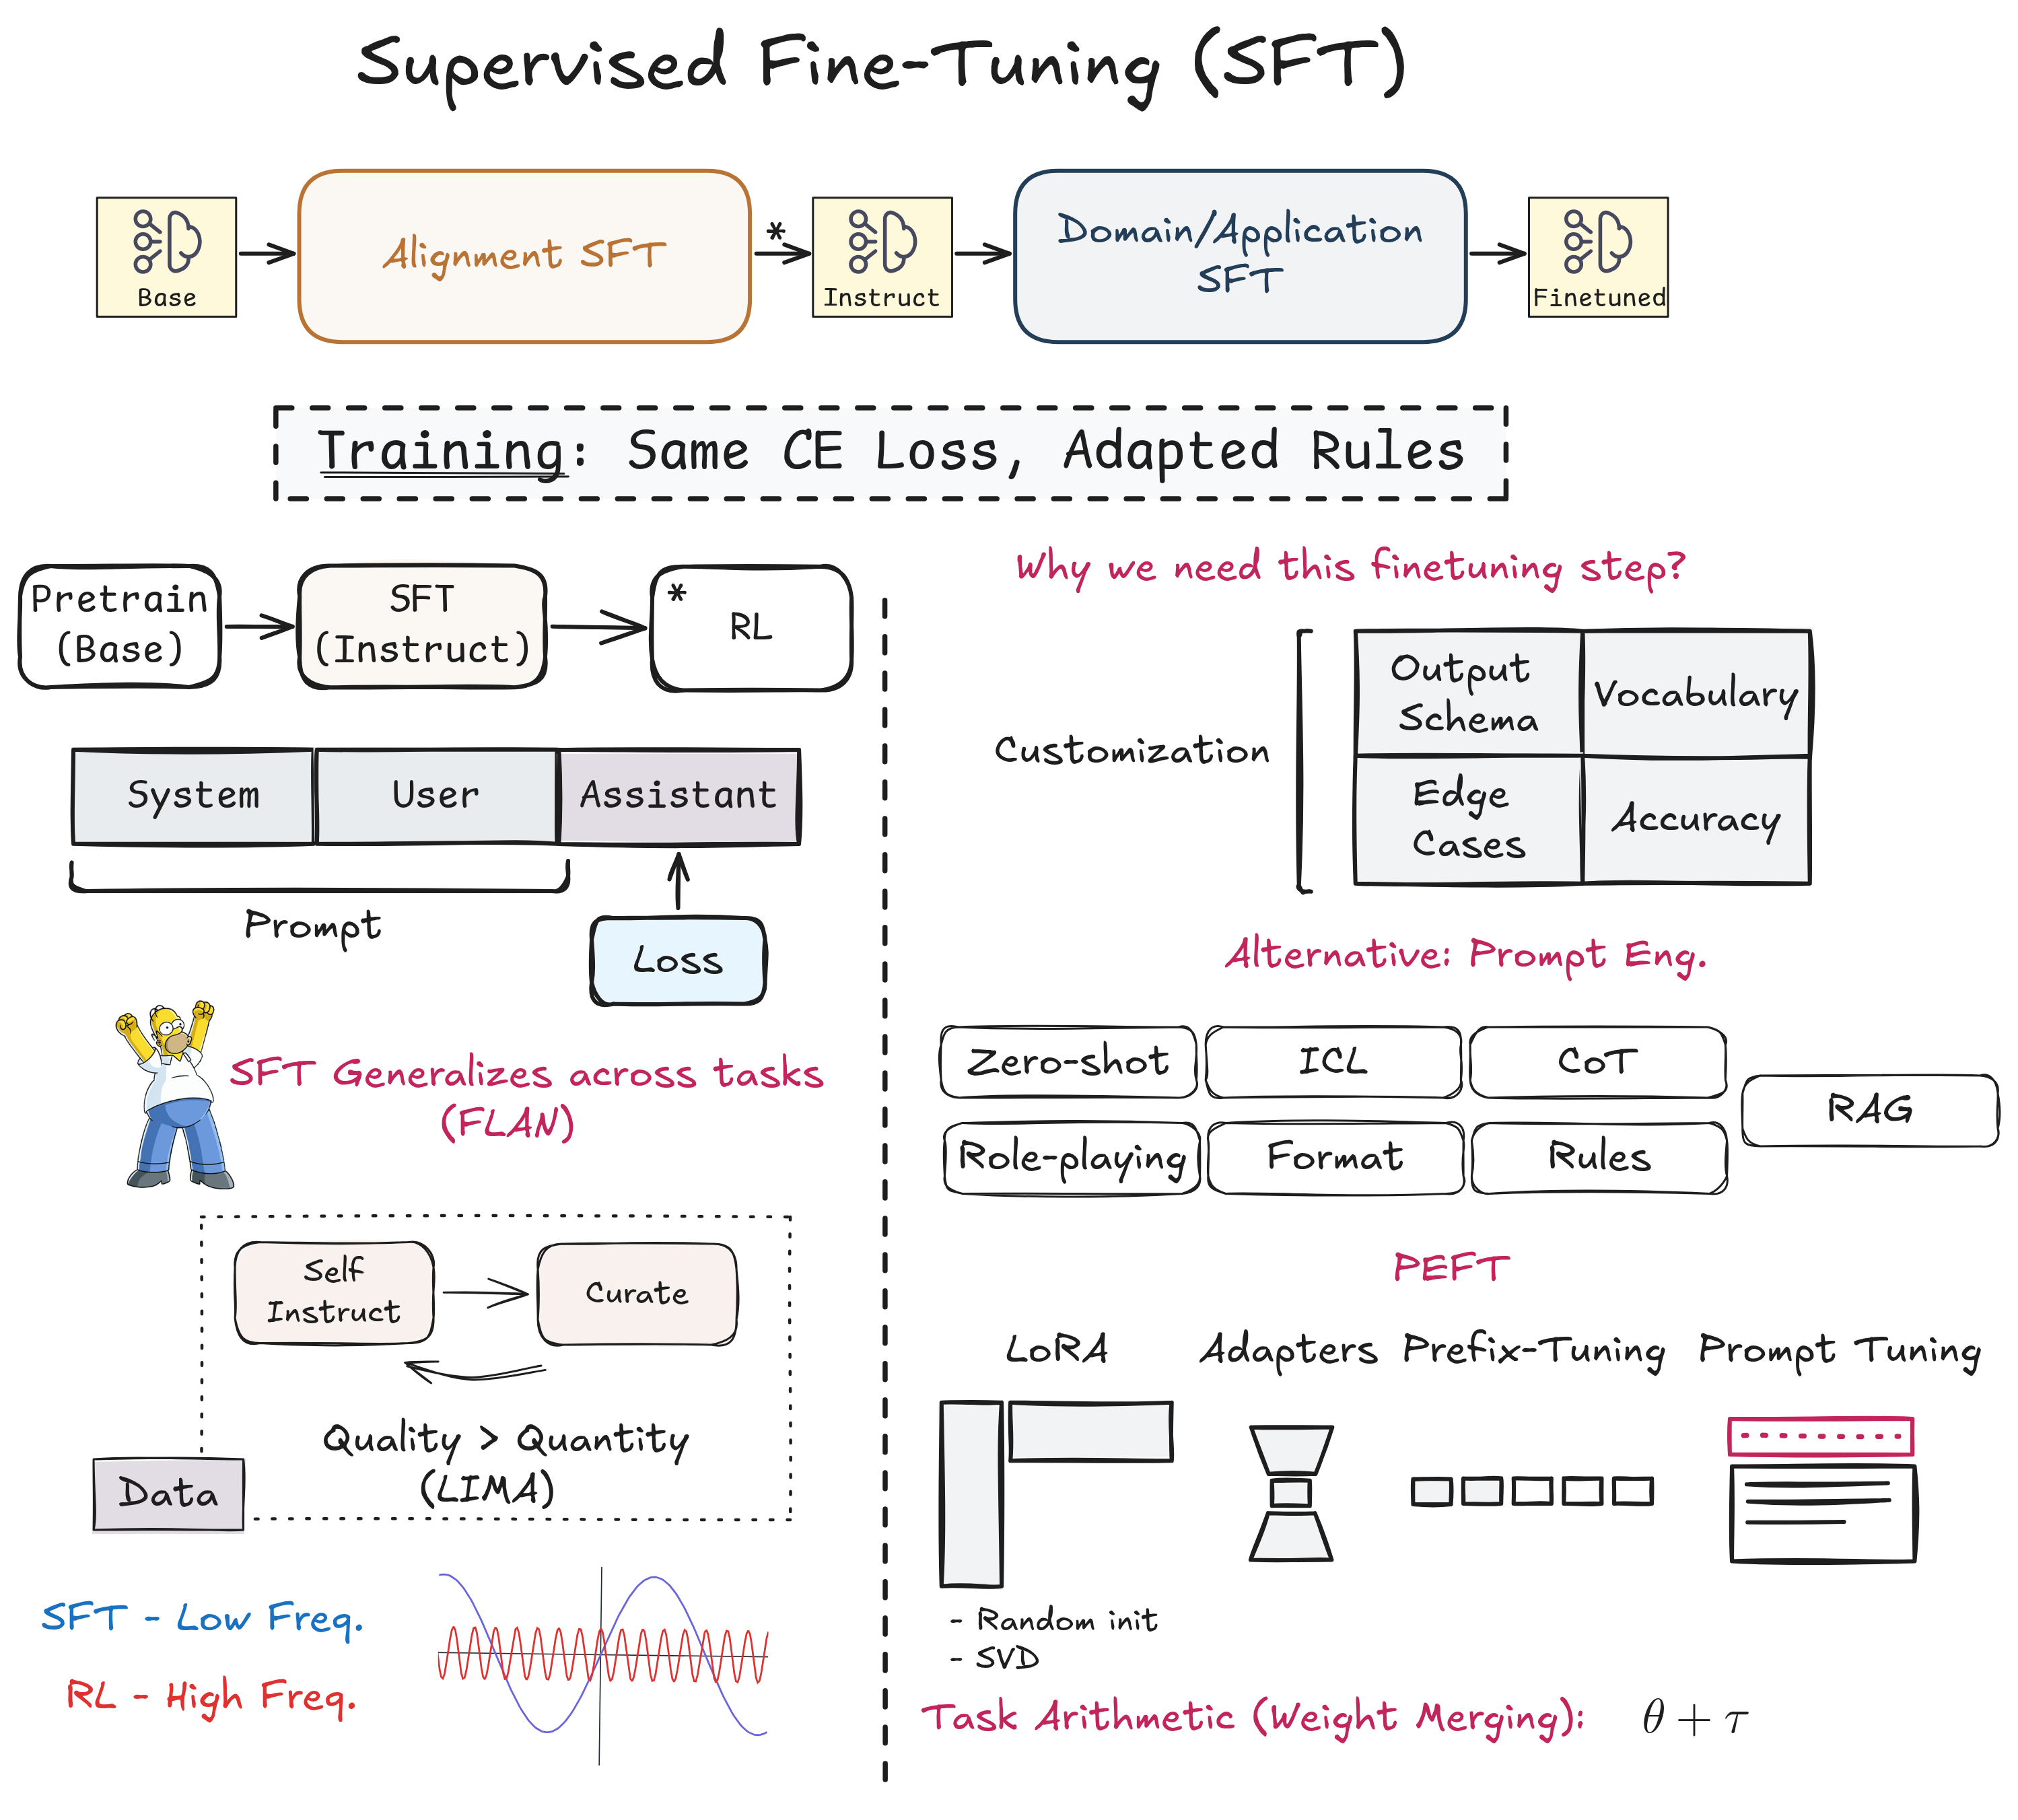
\includegraphics[width=\atlaspanelinnerwidth]{map}};
    \atlasmapcoverbelow{-2.0}
  \end{tikzpicture}
}{\trainingTitle}{\trainingBox}{trainingBodyAnchor}

% ---------------- The LLM Alignment Pipeline ----------------
\begin{frame}{The LLM Alignment Pipeline}
  \begin{center}
  \begin{tikzpicture}[node distance=0.6cm, every node/.style={font=\small}]
    \node[draw, rounded corners, minimum width=3cm, minimum height=1.1cm, align=center] (pre) {Pre-training\\\footnotesize(Base Model)};
    \node[draw, rounded corners, fill=AtlasSlate!20, draw=AtlasSlate, minimum width=3cm, minimum height=1.1cm, align=center, right=of pre] (sft) {SFT\\\footnotesize(Instruction Model)};
    \node[draw, rounded corners, minimum width=3.4cm, minimum height=1.1cm, align=center, right=of sft] (rlhf) {RLHF / DPO\\\footnotesize(Human Preferences)};
    \draw[-Stealth] (pre) -- (sft);
    \draw[-Stealth] (sft) -- (rlhf);
  \end{tikzpicture}
  \end{center}
  \vspace{6pt}
  \begin{itemize}
    \item \textbf{Pre-training:} web-scale raw knowledge and language structure acquisition.
    \item \textbf{SFT:} teaching interaction formats, tasks, and system behaviors.
    \item \textbf{RLHF/DPO:} micro-tuning behavior to meet safety standards and human feedback.
  \end{itemize}
  % >>> FLAGGED -- OPTIONAL ADDITION to an already-reviewed slide (2026-09-07).
  % Delete this \landscapenote line to reject; it only adds a citation, no
  % content change to the diagram/bullets above.
  \landscapenote{\scriptsize This 3-stage pipeline was introduced by Ouyang et al., \emph{Training
  language models to follow instructions with human feedback} (InstructGPT, 2022).}
  % <<< END FLAGGED ADDITION

  \note{
    \footnotesize
    \textbf{RLHF vs. DPO:}\\[3pt]
    \textbf{RLHF} (Reinforcement Learning from Human Feedback) trains a reward model from human preference comparisons, then uses PPO (Proximal Policy Optimization) to fine-tune the language model to maximize that reward. Two-stage process: reward model training, then RL optimization.\\[3pt]
    \textbf{DPO} (Direct Preference Optimization, Rafailov et al., 2023) achieves the same goal --- aligning to human preferences --- but directly optimizes the language model using preference pairs, no separate reward model or RL needed. Single-stage supervised learning on preference data.\\[3pt]
    Both serve the same purpose in the pipeline: refining the SFT model's outputs to match human preferences for helpfulness, harmlessness, and truthfulness. DPO is simpler and often more stable in practice.
  }
\end{frame}

% ---------------- Anatomy of an Instruction Example ----------------
\begin{frame}[fragile]{The Anatomy of an Instruction Example}
  \small
  \textbf{ChatML / OpenAI JSON template structure}
\begin{lstlisting}[language=jsonish]
[
  {"role": "system", "content": "You are a helpful coding assistant."},
  {"role": "user", "content": "How do I reverse a list in Python?"},
  {"role": "assistant", "content": "You can reverse a list using
      `list.reverse()` or slicing `[::-1]`."}
]
\end{lstlisting}
  \vspace{-2pt}
  \begin{center}
  \begin{tikzpicture}[font=\footnotesize]
    \node[draw, fill=NoteGray!15, minimum height=0.6cm, minimum width=1.3cm, align=center] (sys) {System};
    \node[draw, fill=NoteGray!15, minimum height=0.6cm, minimum width=1.3cm, align=center, right=0pt of sys] (usr) {User};
    \node[draw, draw=AtlasCool, fill=AtlasCool!25, minimum height=0.6cm, minimum width=1.6cm, align=center, right=0pt of usr] (asst) {Assistant};
    \draw[decorate, decoration={brace, amplitude=3.5pt, mirror}] ([yshift=-1pt]sys.south west) -- ([yshift=-1pt]usr.south east)
      node[midway, below=5pt, align=center, font=\scriptsize] {\textbf{Prompt} --- context only,\\ \emph{no gradient}};
    \node[draw, rounded corners, fill=white, below=0.85cm of asst] (loss) {Loss $\mathcal{L}$};
    \draw[-Stealth, thick, AtlasCool] (asst.south) -- (loss.north);
  \end{tikzpicture}
  \end{center}
  \vspace{-4pt}
  \slidecaption{\footnotesize \textbf{The Gold Target} --- loss is calculated ONLY on the assistant response.}
  \begin{itemize}[itemsep=1pt,topsep=2pt]
    \item \textbf{System:} defines boundaries/tone.
    \item \textbf{User:} input instructions --- part of the context, not the target.
    \item \textbf{Assistant:} the training target --- this is what the loss actually optimizes.
  \end{itemize}

\end{frame}

\note{
  \footnotesize
  \textbf{Purpose of this slide:} show the audience what a single SFT training example
  physically looks like, and set up the key mechanical fact (loss masking) that the next
  slide's formula depends on.

  \textbf{The code block:} this is the raw JSON that instruction datasets are stored in
  (ChatML / OpenAI's chat format) --- not a diagram, an actual example of the data format.
  Point out it's a list of \{role, content\} turns, concatenated with special template
  tokens (not shown here, kept simple) into one flat sequence before it ever reaches the
  model --- that flattening is what the next slide's $x_1,\dots,x_N$ refers to.
  \begin{itemize}[itemsep=0pt,topsep=2pt]
    \item \textit{system} turn: sets the assistant's persona/behavior for the whole
      conversation --- written once, not something the model is being taught to produce.
    \item \textit{user} turn: the instruction/question --- this is input the model must
      condition on, but never generates itself.
    \item \textit{assistant} turn: the one thing in the whole example the model is actually
      being trained to produce.
  \end{itemize}
}

\note{
  \footnotesize  
  \textbf{Why separate system from user?}\\[3pt]
  The \textit{system} message is persistent context/conditioning that applies to the entire conversation, while \textit{user} messages are per-turn inputs. Separating them allows:\begin{itemize}[itemsep=0pt,topsep=2pt]
    \item \textbf{Persistent behavior:} The system prompt stays active across all turns without repeating it in every user message.
    \item \textbf{Role clarity:} During multi-turn conversations, the model knows which content is meta-instruction (system) vs. actual user input (user).
    \item \textbf{Inference flexibility:} At deployment, you can set the system message once and reuse it across many user queries.
  \end{itemize}

  \textbf{Are they treated differently during training?}\\[3pt]
  Not at the weight-update level --- both system and user tokens are just context (no gradient flows from them due to loss masking). The difference is \emph{implicit} through the tags: the model learns from training data patterns that \texttt{<|system|>} tokens signal persistent conditioning while \texttt{<|user|>} tokens signal per-turn input. The network learns this distinction purely from exposure during training, not from any special algorithmic treatment.

  

}

\note{
  \footnotesize

  \textbf{The role diagram} (gray System+User blocks braced as ``Prompt,'' colored Assistant
  block with an arrow down to Loss): the compressed version of the mechanical rule ---
  system+user together form ``the prompt,'' which is fed in as context; only the assistant
  span contributes to the loss. The arrow deliberately starts \emph{only} at the Assistant
  block --- there is no arrow out of System/User --- so the picture itself says ``no
  gradient from the prompt,'' not just the caption underneath it. Say this out loud as
  ``everything up to the assistant turn is context the model reads; only the assistant turn
  is what it's graded on.''

  \textbf{``The Gold Target'' caption:} names the assistant turn as the \emph{annotation} ---
  i.e.\ this is the ground-truth label a human (or a stronger model) wrote, analogous to a
  label in any supervised-learning setup. Worth explicitly drawing the parallel to
  classification labels here if the audience needs the supervised-learning framing
  reinforced.

  \textbf{Bottom bullets:} restate the three roles in one line each, mapping directly onto
  the code block above --- use these as the actual talking points per role rather than
  re-reading the JSON. The key contrast to land is System+User = context/never a training
  target vs.\ Assistant = the only thing being optimized; this is exactly what ``loss
  masking'' means and is the fact the training-mechanics slide right after this one builds
  on.
}

% ---------------- NEW: Instruction Tuning Generalizes (FLAN) ----------------
\begin{frame}{Instruction Tuning Works: The FLAN Result}
  \small
  \textsc{FLAN --- Finetuned Language Models Are Zero-Shot Learners} (Wei et al., 2022). \\
  \begin{center}
  \textbf{Instruction tuning generalizes across tasks --- not just new examples, but entirely new task types.}
  \end{center}
  \vspace{5pt}

  \begin{center}
  \begin{tikzpicture}[node distance=0.5cm, every node/.style={font=\scriptsize, align=center}]
    \node[draw, rounded corners, minimum width=3.6cm, minimum height=1.1cm] (tasks) {60+ NLP datasets\\(NLI, QA, summ., \ldots)};
    \node[draw, rounded corners, minimum width=3.4cm, minimum height=1.1cm, right=of tasks] (verbalize) {Templated as\\instructions};
    \node[draw, rounded corners, minimum width=2.6cm, minimum height=1.1cm, right=of verbalize, fill=AtlasSlate!20, draw=AtlasSlate] (flan) {FLAN\\137B, instruction-tuned};
    \draw[-Stealth] (tasks) -- (verbalize);
    \draw[-Stealth] (verbalize) -- (flan);
  \end{tikzpicture}
  \end{center}
  \vspace{6pt}

  \begin{noteframe}
    \textbf{Result:} Holding out entire task clusters (e.g., all NLI), zero-shot FLAN beats GPT-3
    on \textbf{20 of 25} held-out types --- even topping few-shot on several.
  \end{noteframe}
  \vspace{4pt}
  {\footnotesize\color{NoteGray} Ablations confirm real generalization: gains grow with task
  diversity and require natural-language phrasing.}

  \note{
    \footnotesize
    \textbf{What this paper is about.} FLAN = ``Finetuned Language Net.'' GPT-3 (2020) showed
    few-shot prompting works but zero-shot is weak. FLAN's fix: instruction-tune a pretrained LM once
    on many tasks phrased as natural-language instructions, so it learns to \emph{follow
    instructions} as a skill, not just continue text.

    \textbf{Method (\S2.1).} 62 labeled NLP datasets (NLI, QA, translation, \ldots) $\to$ 12 task
    clusters $\to$ $\sim$10 hand-written NL templates each. Finetune a 137B LM (LaMDA-PT) on the
    mixture $\to$ FLAN.

    \textbf{Eval (\S2.2--3).} Strict zero-shot: hold out a whole task \emph{cluster} (e.g.\ no NLI at
    all), evaluate on it. Beats zero-shot GPT-3 on 20/25 held-out datasets; beats even few-shot GPT-3
    on ANLI, RTE, BoolQ, ARC, OpenbookQA, StoryCloze.
  }

  \end{frame}

  \note{
    \footnotesize
    \textbf{Why not just multi-task training (\S4.1--4.3).} (a) more clusters keeps helping, not
    saturated; (b) only works at scale --- \emph{hurts} models $\leq$8B (capacity goes to memorizing
    the $\sim$40 tasks, not generalizing); (c) dropping the instructions (raw I/O, or a dataset-name
    tag) performs much worse --- the phrasing itself is what's doing the work.

    \textbf{GPT-3 caveat.} GPT-3 (Brown et al., 2020) is a \textbf{base model only} --- pretrained on web text, no instruction tuning. It was evaluated purely via \textbf{prompting strategies}: zero-shot (task description only), one-shot (1 example), and few-shot (typically K=10-100 in-context examples prepended to the prompt). No gradient updates, no fine-tuning.\\[3pt]
    \textbf{How the comparison worked:} FLAN's zero-shot performance (instruction-tuned model, no examples) was compared against GPT-3's zero-shot and few-shot ICL (base model with K examples in-context). The base model GPT-3 \emph{could} follow instructions when given enough in-context examples showing the pattern --- this is what ICL/prompting engineering exploits. FLAN's contribution: instruction tuning eliminates the need for those per-query examples.\\[3pt]
    InstructGPT (Ouyang et al., 2022, on the Pipeline slide) applies SFT+RLHF to GPT-3 a year later. FLAN beats the \emph{prompting-only} paradigm of its time, not a rival instruction-tuned model.
  }

  \note{
    \footnotesize
    \textbf{Actual contribution:} not the benchmark numbers, and not FLAN's data-sourcing trick
    (repurposed datasets --- not how modern pipelines source SFT data, see next slides). It's proof
    instruction tuning itself induces real generalization to unseen human--model interactions.
  }


% ---------------- NEW: Bootstrapping Instructions from the Model Itself (Self-Instruct) ----------------
\begin{frame}{Bootstrapping Instructions from the Model Itself: Self-Instruct}
  \small
  \textsc{Self-Instruct} (Wang et al., 2023). \\
  \begin{center}
    \textbf{Have the model generate its own training data, then filter.}
  \end{center}
  \vspace{5pt}

  \begin{center}
  \begin{tikzpicture}[node distance=0.4cm and 0.25cm, every node/.style={font=\tiny, align=center, text width=2.3cm}, arr/.style={-{Stealth[length=4pt]}}]
    \node[draw, rounded corners, minimum height=0.9cm] (seed) {Seed tasks\\(175 human-written)};
    \node[draw, rounded corners, minimum height=0.9cm, right=of seed] (gen) {Generate new\\instruction data};
    \node[draw, rounded corners, minimum height=0.9cm, right=of gen] (filt) {Filter\\(quality \& novelty)};
    \node[draw, rounded corners, minimum height=0.9cm, right=of filt, fill=AtlasSlate!20, draw=AtlasSlate] (ft) {Fine-tune\\same model};
    \draw[arr] (seed) -- (gen);
    \draw[arr] (gen) -- (filt);
    \draw[arr] (filt) -- (ft);
    \draw[arr, dashed] (filt.north) to[out=100,in=80] node[midway, above, text width=2.6cm]{iterates} (gen.north);
  \end{tikzpicture}
  \end{center}
  \vspace{6pt}

  \begin{noteframe}
    \textbf{Result:} $+$33.1\% ROUGE-L over GPT-3 on Super-NaturalInstructions --- within 5\% of
    InstructGPT on novel tasks, minimal annotation.
  \end{noteframe}

  \landscapenote{Direct ancestor of the Llama 3 rejection-sampling pipeline (two slides ahead) ---
  less refined.}

  \end{frame}

  \note{
    \footnotesize
    \textbf{Purpose:} closes the ``where does instruction data come from'' arc opened by FLAN ---
    FLAN reused existing labeled datasets; Self-Instruct bootstraps from the model's own
    generations instead. Wang et al.\ 2023: 175 seed tasks, iteratively expanded, +33.1\% ROUGE-L
    over vanilla GPT-3 on Super-NaturalInstructions, within 5\% of InstructGPT\textsubscript{001}.

    \textbf{What are the seed tasks?} 175 manually written (instruction, input, output) triplets covering diverse categories (e.g., generation, classification, editing, QA). Each seed task is a complete example showing: an instruction (``Write a haiku about nature''), optional input context (could be empty), and a correct output (the haiku itself).\\[3pt]
    \textbf{How are they used?} As \textbf{in-context examples in the generation prompt}. At each iteration, the model is prompted with: (1) a short meta-instruction explaining the task-generation goal, (2) a random sample of K existing tasks (initially from the 175 seeds, later includes previously generated tasks), (3) ``Generate a new instruction:\textbackslash n''. The model completes this prompt with a new instruction triplet. This is pure ICL --- no gradient updates during generation, just few-shot prompting off the seed pool.\\[3pt]
    

  }

  \note{
    \footnotesize
    \textbf{What prompt format?} Meta-prompt template from \S2: ``You are asked to come up with a set of diverse task instructions\ldots Here are some examples:\textbackslash n [K sampled tasks] \textbackslash n Now generate a new task:\textbackslash n''. The model (GPT-3 text-davinci-003 in the paper) generates the new instruction as a text completion.

    \textbf{ROUGE-L:} Recall-Oriented Understudy for Gisting Evaluation, Longest Common Subsequence
    variant --- measures text overlap between generated and reference outputs by finding the longest
    matching word sequence (order-sensitive, unlike unigram ROUGE). Ranges 0--100; higher is better.
    SuperNI (Super-NaturalInstructions) uses ROUGE-L because it tests diverse generation tasks, not
    just classification. Vanilla GPT-3's 6.8 means its zero-shot outputs barely overlap with the
    gold references; Self-Instruct's 39.9 shows real instruction-following ability.

    \textbf{The filter, precisely (\S2):} three cheap automatic checks, none of which verify
    correctness. \emph{Diversity:} new instruction kept only if ROUGE-L vs.\ every existing
    instruction is $<0.7$ (catches near-dupes, not wrong answers). \emph{Keyword filter:} drop
    instructions needing images/graphs a text-only LM can't do. \emph{Instance heuristics:} drop
    exact-dup instances, same-input-conflicting-output pairs, and too-long/short or
    input-repeating outputs. No reward model, no human judgment, no correctness check anywhere.
  }

  \note{
    \footnotesize
    \textbf{Is the data actually correct? No (\S3.3).} 200 sampled instructions, human-graded:
    92\% valid instruction, only 58\% correct output, only \textbf{54\% fully valid end to end}
    --- shipped anyway (``the value of the generated data despite the noise''). One-time
    diagnostic, not a real filter. Bet: CE-loss SFT tolerates a noisy minority, partial-correctness
    still teaches format, and quality is raised \emph{later} via iteration/distillation (re-scoring
    outputs with InstructGPT\textsubscript{003} lifted results 10\%) rather than guaranteed upfront.

    \textbf{Delivery:} land the shift from \emph{curated-by-humans} (FLAN) to
    \emph{generated-by-model, filtered-by-rules} (Self-Instruct) --- pushed further with much
    stricter filtering on the Llama 3 slide next. If asked about correctness guarantees: no ---
    the 54\%-valid number above is the honest answer; both pipelines accept noise rather than
    hand-validating every example.
  }


% ---------------- NEW: Where the Data Actually Comes From (Llama 3 / DeepSeek-V3) ----------------
\begin{frame}{Where the Data Actually Comes From}
  \footnotesize
  \begin{center}
  \textbf{Both reports use mostly model-generated data --- humans verify or select, not write from
  scratch.}
  \end{center}
  \vspace{2pt}

  \begin{columns}[t]
    \column{0.5\textwidth}
      \begin{warmbox}
        \footnotesize
        \textbf{\color{AtlasWarm}DeepSeek-V3 --- Model Generates, Humans Verify}
        \begin{itemize}[itemsep=1pt,topsep=2pt]
          \item \textbf{Reasoning} (math/code/logic): generated by \textbf{DeepSeek-R1}, an internal
            AI reasoning model, then rejection-sampled.
          \item \textbf{Non-reasoning} (writing, role-play, QA): generated by \textbf{DeepSeek-V2.5};
            humans \emph{verify} correctness, don't write it.
        \end{itemize}
      \end{warmbox}
    \column{0.5\textwidth}
      \begin{coolbox}
        \footnotesize
        \textbf{\color{AtlasCool}Llama 3 --- Humans Write Prompts, Models Draft Responses}
        \begin{itemize}[itemsep=1pt,topsep=2pt]
          \item \textbf{Prompts:} collected via human annotation --- real-world-style use cases.
          \item \textbf{Responses:} mostly \textbf{rejection-sampled} ($K{=}10$--30, RM picks best)
            --- not human-written.
          \item Plus targeted \textbf{synthetic data} (code, long-context, tools) and a small
            hand-curated slice.
        \end{itemize}
      \end{coolbox}
  \end{columns}
  \vspace{4pt}

  \landscapenote{\footnotesize Both pipelines diverge from FLAN: humans supply prompts, models
  draft responses, then filter via sampling or verification.}


\end{frame}

  \note{
    \footnotesize
    \textbf{Purpose:} the concrete, production-scale answer to ``where does the data come from,''
    using the same two reports the deck treats as verified sources elsewhere (DeepSeek-V3/Llama 3
    case studies two slides ahead cover \emph{quality}, not sourcing).

    \textbf{Sources.} DeepSeek-V3 Tech.\ Report \S5.1: reasoning data (math/code/logic) generated by
    an internal DeepSeek-R1 expert model (own SFT+RL pipeline), rejection-sampled into the final mix;
    non-reasoning data generated by DeepSeek-V2.5, human-verified for correctness. Llama 3 Herd of
    Models \S4.2.1--4.2.2 (Table 6/7): prompts collected via human annotation; SFT responses mostly
    rejection-sampled ($K{=}10$--30, RM picks best), plus targeted synthetic data where hand-annotation
    is impractical (e.g.\ 38K-token long-context examples) and a small hand-curated slice.

    \textbf{Delivery:} contrast with FLAN --- FLAN assumed labeled datasets already existed; neither
    lab has that luxury for an open-ended assistant, so both converge instead on: humans supply/vet
    \emph{prompts}, a model drafts \emph{responses}, rejection sampling or human review filters. Direct
    descendant of Self-Instruct's generate-then-filter loop (previous slide), just industrialized.
  }

\note{
    \footnotesize
    \textbf{Why DeepSeek separates reasoning vs. non-reasoning:} Different generation strategies and quality bars. \textbf{Reasoning tasks} (math/code/logic) have verifiable correctness --- you can check if code runs or math is right --- so they use DeepSeek-R1, a model trained with RL specifically for multi-step reasoning, and filter via rejection sampling against those checks. \textbf{Non-reasoning tasks} (writing, QA, roleplay) have no automatic correctness test, so they generate with DeepSeek-V2.5 (a general model) and rely on human verification instead.\\[3pt]
    \textbf{What is RM (Reward Model)?} A separate neural network trained to score how good a model's response is, based on human preference comparisons. Given (prompt, response) pairs labeled by humans as better/worse, the RM learns to predict a scalar reward. Used during rejection sampling to pick the best candidate out of K generations.\\[3pt]
    \textbf{What is rejection sampling and what is K?} Generate K different responses to the same prompt (K=10--30 in Llama 3), score all K with the RM, keep only the highest-scoring one as the training target. This filters out low-quality generations without human review per example. K is the sample budget: higher K = better chance of getting a good response, but K$\times$ inference cost.\\[3pt]
}

\note{
    \footnotesize
    
    \textbf{What is synthetic data in Llama 3?} Model-generated examples for tasks where human annotation is impractical. Examples: code (generate thousands of coding problems + solutions programmatically), long-context (38K-token examples that would take hours to write by hand), tool use (function-calling demonstrations scripted rather than collected from real users). Still filtered/verified, but the prompt-response pair originates from code or another model, not a human writing both sides.
  }

% ---------------- Two Data Regimes ----------------
\begin{frame}{DeepSeek-V3: Quantity vs.\ Quality, by the Numbers}
  \noindent{\small\itshape A case study from one published model report --- {\color{AtlasWarm}DeepSeek-V3}.}
  \vspace{4pt}

  \begin{center}
  \footnotesize
  \def\arraystretch{1.05}
  \begin{tabular}{lp{4.0cm}p{4.2cm}}
    \toprule
    \textbf{Stage} & \textbf{Data} & \textbf{Compute} \\
    \midrule
    Pre-training & 14.8T tokens & 2{,}664K H800-hrs $\rightarrow$ \$5.33M \\
    Context extension & YaRN, 2 phases $\times$ 1000 steps: 4K$\to$32K$\to$128K & 119K H800-hrs $\rightarrow$ \$0.24M \\
    Post-training (SFT+RL) & 1.5M instruction instances & 5K H800-hrs $\rightarrow$ \$0.01M \\
    \bottomrule
  \end{tabular}
  \end{center}
  {\scriptsize\color{NoteGray}Context extension: no new data, just longer sequences --- the model re-learns to attend over a longer window before it's taught to follow instructions.  \emph{Caveat: the post-training figure bundles SFT and RL; no SFT-only cost is published.}}

  \vspace{6pt}
  \begin{center}
  {\scriptsize\color{NoteGray}\textsc{DeepSeek-V3 at a glance} --- MoE, 671B total / 37B active params $\cdot$ 128K-token context $\cdot$ 128K BPE vocabulary}
  \end{center}

  \note{
    \footnotesize
    \textbf{Purpose:} land one number-backed contrast before the mechanics --- pre-training and SFT
    run the \emph{same} loss on the \emph{same} model, but on data from opposite regimes. This slide
    stays inside a single report so every ratio is an apples-to-apples comparison; the next slide
    switches to Llama 3 to show \emph{how} curation is actually done.

    \textbf{Sources.} DeepSeek-V3 Technical Report, Table 1 (\S1) --- 2664K / 119K / 5K H800 GPU-hours
    for pre-training / context extension / post-training, priced at \$2 per H800 GPU-hour, \$5.576M
    total. Pre-training data: \S4 (14.8T ``high-quality and diverse tokens''). Context extension:
    \S4.3 --- YaRN, two 1000-step phases, 4K$\to$32K then 32K$\to$128K. SFT data: \S5 --- ``we
    curate our instruction-tuning datasets to include 1.5M instances spanning multiple domains.''
    Model specs: \S1/\S4.1 --- MoE, 671B total / 37B active params, 128K context, 128K BPE vocab.

    \textbf{What is YaRN?} YaRN (``Yet another RoPE extensioN,'' Peng et al., 2023) is a method for extending the context window of transformer models that use RoPE (Rotary Position Embeddings). Models are typically pretrained with a fixed maximum sequence length (here, 4K tokens). To handle longer contexts without full retraining, YaRN modifies the RoPE frequency parameters to interpolate position encodings beyond the original training range.\\[3pt]
    \textbf{How it works:} RoPE encodes position information by rotating token embeddings based on their position in the sequence. YaRN applies a non-uniform scaling to different frequency dimensions --- high-frequency components (which capture fine-grained positional distinctions) are preserved, while low-frequency components (which encode coarse position) are scaled down to accommodate longer distances. This lets the model generalize to longer sequences with minimal additional training.\\[3pt]
    \textbf{DeepSeek's two-phase approach:} First phase continues training for 1000 steps at 4K$\to$32K (8$\times$ extension), then second phase for another 1000 steps at 32K$\to$128K (4$\times$ extension). Total cost is minimal (119K H800-hours, vs. 2664K for pretraining) because you're only teaching the model to attend over longer windows using the \emph{same} pretraining data, not learning new knowledge. Same learning rate as the end of pretraining.

    \textbf{Delivery:} read the ratio, not the digits --- 500$\times$ and seven orders of magnitude
    are the point; the exact GPU-hours just show it's a real reported figure, not a hand-wave.

    \textbf{Caveat:} nobody publishes an SFT-only budget --- production pipelines interleave SFT
    and RL, so ``post-training is cheap'' is honest at the stage level, not per-algorithm. Next
    slide: if it's that cheap, what's actually hard about it?
  }
\end{frame}

% ---------------- What "Curated" Actually Means ----------------
\begin{frame}{What ``Curated'' Actually Means}
  \noindent{\small\itshape A case study from one published model report --- {\color{AtlasWarm}Llama 3}.}
  \footnotesize
  \begin{columns}[t]
    \column{0.5\textwidth}
      \begin{warmbox}
      \textbf{\color{AtlasWarm}Pre-training Data}\\[1pt]
      {\scriptsize Scraped from the web --- \textsc{bulk, automatic, corpus-level}}
      \begin{center}
      \vspace{4pt}
      \begin{tikzpicture}[
          font=\tiny,
          every node/.style={align=center, text width=3.1cm},
          node distance=7pt and 0pt,
          arr/.style={-{Stealth[length=4pt]}}
        ]
        \node (l1) {Dedup (URL / doc via MinHash / line)};
        \node (l2) [below=of l1] {Heuristic filters (n-grams, dirty words, KL)};
        \node (l3) [below=of l2] {fastText / RoBERTa classifiers};
        \draw[arr] (l1.south) -- (l2.north);
        \draw[arr] (l2.south) -- (l3.north);
      \end{tikzpicture}
      \end{center}
      \end{warmbox}

    \column{0.5\textwidth}
      \begin{warmbox}
      \textbf{\color{AtlasWarm}SFT Data}\\[1pt]
      {\scriptsize Written/generated on purpose --- \textsc{per-example, model-judged}}
      \begin{center}
      \vspace{4pt}
      \begin{tikzpicture}[
          font=\tiny,
          every node/.style={align=center, text width=3.1cm},
          node distance=7pt and 0pt,
          arr/.style={-{Stealth[length=4pt]}}
        ]
        \node (r1) {Rejection sampling ($K{=}10$--$30$)};
        \node (r2) [below=of r1] {Clean \& topic-tag};
        \node (r3) [below=of r2] {Quality $\times$ difficulty score};
        \node (r4) [below=of r3] {Semantic dedup};
        \draw[arr] (r1.south) -- (r2.north);
        \draw[arr] (r2.south) -- (r3.north);
        \draw[arr] (r3.south) -- (r4.north);
        \draw[decorate, decoration={brace, amplitude=4pt, raise=2pt}, AtlasCool, thick]
          (r1.north east) -- (r4.south east)
          node[midway, xshift=32pt, text width=1.4cm, align=left, color=AtlasCool]
          {\textbf{$\times$6}\\ rounds};
      \end{tikzpicture}
      \end{center}
      \end{warmbox}
  \end{columns}
  \vspace{-3pt}
  \landscapenote{\scriptsize Llama 3's own summary: \emph{``more careful pre-processing and curation pipelines for pre-training data $\ldots$ more rigorous quality assurance and filtering approaches for post-training data.''} \S3.1 / \S4.2.3.}

  \end{frame}
  
  \note{
    \footnotesize
    \textbf{Purpose:} both columns are Llama 3 alone --- shows \emph{how} its ``more rigorous''
    claim is implemented, step by step.

    \textbf{Left (\S3.1):} \emph{Dedup} --- URL/line matching + MinHash. \emph{Heuristic filters}
    --- n-gram/dirty-word counts flag spam; token-distribution KL flags non-natural-language text.
    \emph{fastText/RoBERTa classifiers} --- learned scorers (RoBERTa trained on Llama 2's own
    quality judgments) keep only higher-quality pages.

    \textbf{What are fastText and RoBERTa classifiers?}\\[3pt]
    \textbf{fastText} (Joulin et al., 2016): Lightweight text classifier from Facebook. Represents documents as bag-of-n-grams, learns linear weights via SGD. Fast ($\sim$millions of docs/hour on CPU), used here as a first-pass quality filter to score pages before the slower RoBERTa pass.\\[3pt]
    \textbf{RoBERTa} (Liu et al., 2019): BERT-based transformer encoder, trained on masked language modeling. Fine-tuned here on Llama 2's human quality annotations to predict "is this page high-quality enough for pre-training?" as a binary/regression task. Slower but more accurate than fastText --- only runs on fastText-passed docs.

  }

  \note{
    \footnotesize


    \textbf{Right (\S4.2.3):} \emph{Rejection sampling ($K{=}10$--$30$)} --- per prompt, sample $K$
    outputs from the current best chat checkpoint, RM scores all $K$, keep the top pick; later
    rounds add system prompts to steer tone before scoring. \emph{Clean \& topic-tag} --- rules +
    a fine-tuned Llama 3 8B classifier.
    \emph{Quality$\times$difficulty} --- RM top-quartile score $\times$ Instag difficulty, so hard
    examples survive. \emph{Semantic dedup} --- RoBERTa clustering removes near-copies. Whole chain
    repeats \textbf{6 rounds}, each round's model generating the next round's candidates.

    \textbf{How each SFT curation step works:}\\[3pt]
    \textbf{Clean \& topic-tag:} Rule-based text cleaning (remove malformed Unicode, fix formatting), then a fine-tuned Llama 3 8B model classifies each example into topic categories (code, math, creative writing, etc.). Both automated --- no human per-example review.\\[3pt]
    \textbf{Quality $\times$ difficulty score:} Two model-based scores multiplied together. (1) \emph{Quality}: RM (reward model) scores each response, keep only top quartile. (2) \emph{Difficulty}: Instag (instruction tagging model) estimates prompt complexity/ambiguity. Product ensures we keep high-quality responses to hard prompts, not just easy wins.\\[3pt]

  }

  \note{
    \footnotesize
    \textbf{Semantic dedup:} Embed all responses with RoBERTa, cluster by cosine similarity, drop near-duplicates within each cluster. Removes paraphrases/near-copies that would waste SFT capacity, keeping only one representative per semantic bucket. All model-based --- no human clustering.
    
    \textbf{Secretly RL?} Yes: best-of-$K$-then-imitate is the same family as best-of-N policy
    improvement / STaR / RAFT / ReST --- RM picks the best current-policy sample, SFT imitates it.
    \emph{Not} PPO/DPO-style: no gradient through reward/sampling, no value function, and
    top-1-of-$K$ discards all reward signal below the winner --- ``RL-flavored data generation
    feeding a supervised objective.''

    \textbf{Guarantees correct data? No.} Humans mainly verify prompts/preference pairs, not every
    SFT sample --- a statistical filter at scale, not a per-example guarantee (the paper admits its
    RM- and Llama-based scores ``have high disagreement rates''). Same bet as Self-Instruct,
    stricter and iterated 6$\times$: tolerate noise, raise quality via iteration.

    \textbf{Delivery:} name the funnel shape (bulk/automatic left vs.\ model-judged right); hold
    RL-framing/no-guarantee point in reserve for questions.
  }


% ---------------- LIMA Effect ----------------
\begin{frame}{Quality Over Quantity: The LIMA Effect}
  \small
  \textbf{LIMA (Zhou et al., 2023): 1,000 curated examples outperform Alpaca's 52K and stay competitive with RLHF'd models like DaVinci003 and Bard.}
  \vspace{5pt}

  \begin{noteframe}
    \textbf{Equal-or-Preferred Rate} --- \% of matchups where LIMA tied or won in blind comparisons.
  \end{noteframe}
  \vspace{6pt}

  \begin{center}
  \footnotesize
  \def\arraystretch{1.15}
  \begin{tabular}{lcccc}
    \toprule
    \textbf{vs.\ baseline} & \textbf{DaVinci003 (RLHF)} & \textbf{Bard} & \textbf{Claude} & \textbf{GPT-4} \\
    \midrule
    LIMA equal-or-preferred & \textbf{65\%} & \textbf{58\%} & 46\% & 43\% \\
    \bottomrule
  \end{tabular}
  \end{center}

  \landscapenote{65B LLaMA, 1,000 examples, no RLHF.}

  \note{
    \footnotesize
    \textbf{Full context (condensed from slide).} LIMA is a 65B LLaMA model fine-tuned on just
    1,000 meticulously curated prompt/response pairs, with no RLHF at all. It beats a
    52$\times$-larger, uncurated set (Alpaca's 52{,}000 self-instruct examples) and stays
    competitive with RLHF'd frontier models. The core takeaway: quantity alone doesn't buy
    alignment quality --- careful curation matters more than dataset size.

    \textbf{Equal-or-Preferred Rate (full definition).} Annotators see two anonymous responses per
    prompt and pick the better one, or call it a tie. ``$X\%$ equal-or-preferred'' means LIMA tied
    or won in $X\%$ of matchups.

    \textbf{Sources.} Zhou et al., \emph{LIMA: Less Is More for Alignment} (2023), \S4.2 / abstract
    --- equal-or-preferred rates: 65\% vs.\ DaVinci003, 58\% vs.\ Bard, 46\% vs.\ Claude, 43\% vs.\
    GPT-4. Alpaca comparison (52{,}000 self-instruct examples, not raw web data) is qualitative in
    the paper --- no exact \% given, so it's stated as text above rather than in the table.

    \textbf{Delivery:} the punchline up top is the actual takeaway --- LIMA doesn't uniformly
    ``win,'' it's \emph{competitive} despite 1--2 orders of magnitude less data and no RLHF. Don't
    oversell the table as LIMA beating everyone; it loses more often than not to Claude/GPT-4, just
    not by a landslide.
  }

\end{frame}

% >>> FLAGGED -- OPTIONAL SLIDE (2026-09-07). Sits just past the requested
% Pipeline-to-LIMA range: it's a bridge out of Alignment SFT into whatever
% RLHF/DPO content follows. Delete this whole \begin{frame}...\end{frame}
% block to reject it without touching anything else.
% ---------------- After SFT: Why RL Still Helps ----------------
\newcommand{\rlStillHelpsTitle}{After SFT: Why RL Still Helps}
\newsavebox{\rlStillHelpsBox}
\newcommand{\rlStillHelpsBody}{%
  \small
  \begin{columns}[t]
    \column{0.5\textwidth}
      \begin{warmbox}
        \textbf{\color{AtlasWarm}Alignment SFT}\\[2pt]
        Instruction-following, persona\\[4pt]
        {\scriptsize\color{NoteGray} Broad behavioral patterns\\
        Overfits to training details}
      \end{warmbox}
    \column{0.5\textwidth}
      \begin{coolbox}
        \textbf{\color{AtlasCool}RL / RLHF}\\[2pt]
        Preferences, refusals, style\\[4pt]
        {\scriptsize\color{NoteGray} Fine-grained calibration\\
        Adapts to variation}
      \end{coolbox}
  \end{columns}
  \vspace{10pt}

  \begin{noteframe}
    \textbf{SFT stabilizes format; RL calibrates boundaries.}
  \end{noteframe}

  \landscapenote{\scriptsize SFT captures \textbf{low-frequency patterns} (instruction-following), RL calibrates \textbf{high-frequency variation} (preferences, refusals, style) --- complementary. TailSFT (Malladi et al., 2026) filters well-fit sequences, improving pass@K for RL.}

}
\atlasslide{\rlStillHelpsTitle}{\rlStillHelpsBox}{rlStillHelpsBodyAnchor}{\rlStillHelpsBody}

% ---------------- Map-return: back to the RL Still Helps slide's map ----------------
\atlasmapreturn[0.6]{}{%
  \begin{tikzpicture}
    \node[anchor=north west, inner sep=0pt] (img) {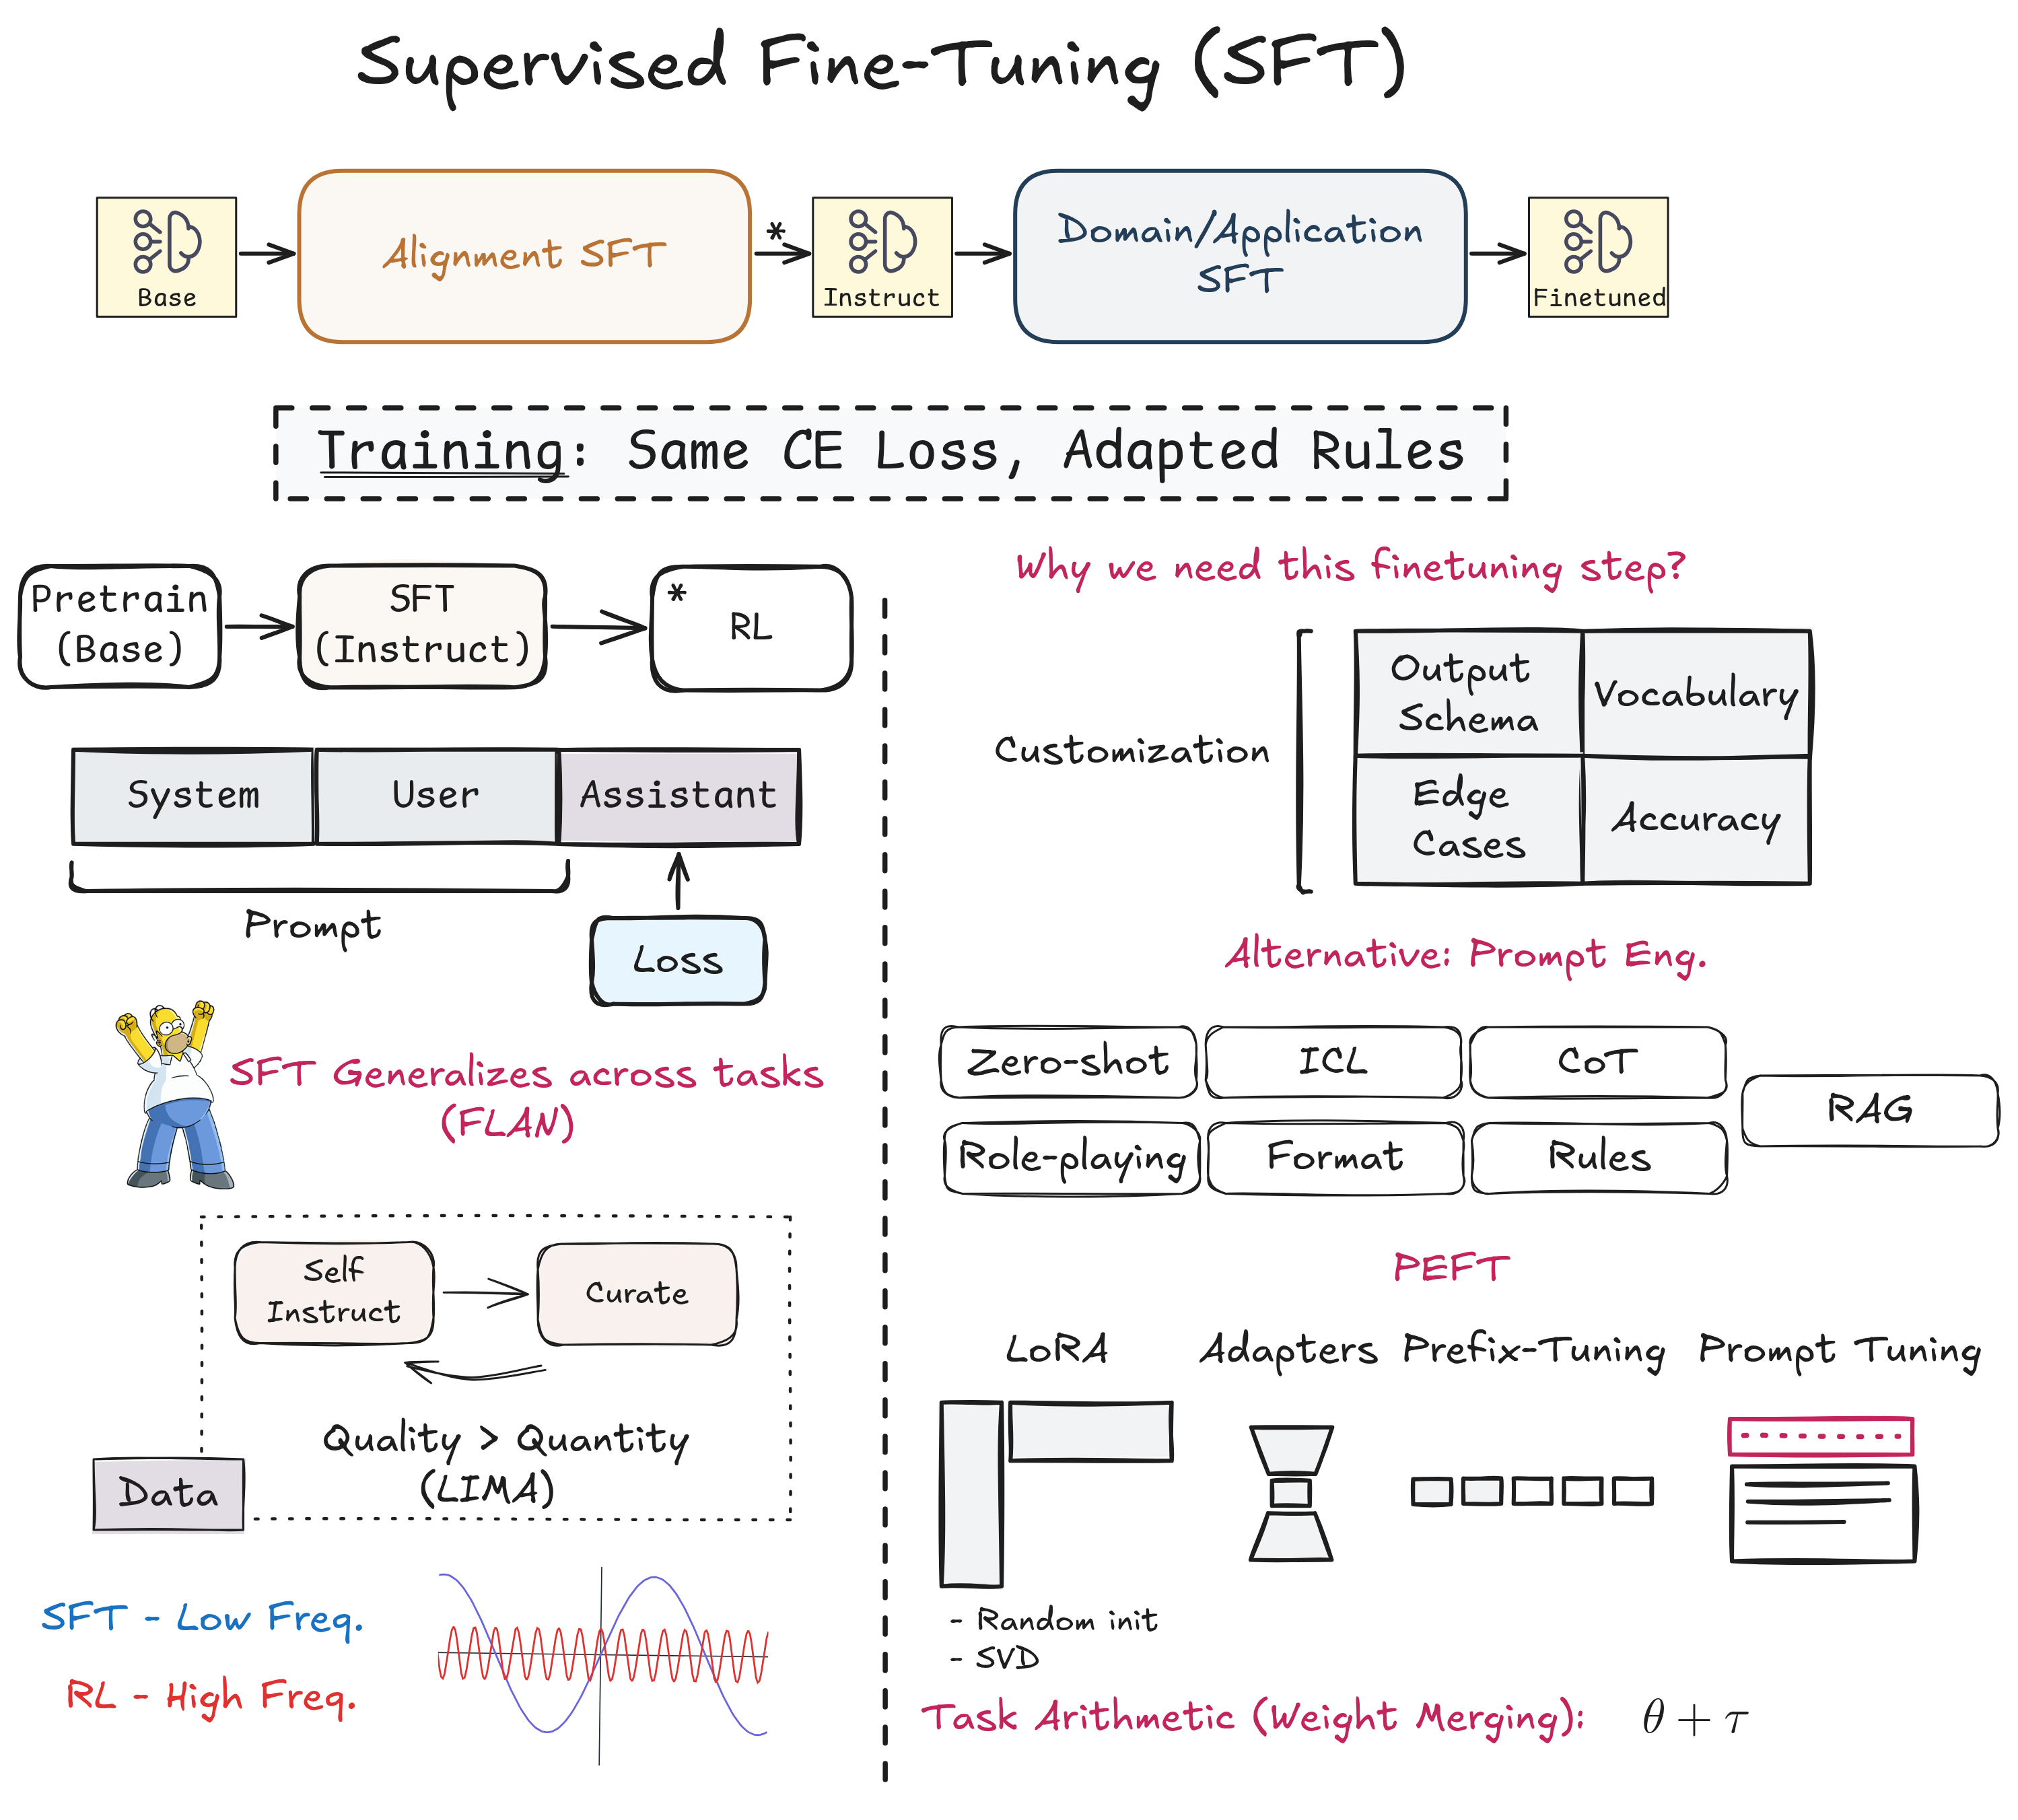
\includegraphics[width=\atlaspanelinnerwidth]{map}};
    % Cover bottom-right corner: from middle to right edge, same height as old bottom covering
    \atlasmapcover{0.45\atlaspanelinnerwidth}{-50cm}{\atlaspanelinnerwidth}{-2.0cm}
  \end{tikzpicture}
}{\rlStillHelpsTitle}{\rlStillHelpsBox}{rlStillHelpsBodyAnchor}

\note{
    \footnotesize
    \textbf{Slide structure.} This slide has two parts: first, concrete bullets showing what each training stage teaches; second, the frequency-domain reframe that explains \emph{why} we need both. The bullets give grounding; the frequency lens gives the underlying principle.

    \textbf{The frequency analogy (yours, not Chu's direct claim).} Low-frequency = broad patterns evident across diverse examples; high-frequency = fine-grained calibration at the margins. SFT learns from fixed demonstrations --- it can only interpolate within patterns it saw. RL learns from reward signals --- it can explore and calibrate based on feedback.
}

\note{
    \textbf{Why preference/refusal/style map to high-frequency:}
    \begin{itemize}
      \item \textbf{Preference alignment:} What counts as ``better'' varies by context, user, subtle phrasing --- not a fixed pattern SFT can memorize from demonstrations.
      \item \textbf{Refusal boundaries:} The refuse/comply decision depends on fine-grained context; SFT examples can't cover every edge, but RL's feedback loop can calibrate where the boundary sits.
      \item \textbf{Response style:} Tone, verbosity, formatting preferences vary across situations --- RL tunes these calibrations to human feedback in ways SFT's fixed demos can't capture.
    \end{itemize}
    Unifying idea: SFT teaches the broad ``be a helpful assistant'' pattern; RL tunes the quality/boundary/style decisions that vary too much to capture in fixed training examples. It's calibration at the edges, not learning the behavior itself.
  }

  \note{
    \footnotesize
    \textbf{Caveat for defending the analogy:} This is a pedagogical frame, not a theorem. The Chu et al. experiments showed SFT overfitting to training specifics (rule/visual details) while RL adapted to unseen variants --- the mapping to preference/refusals/style is conceptual but defensible. The boundary isn't perfectly clean (SFT learns some details, RL reinforces some broad patterns), but as a frame for ``why do we need RL after SFT,'' it holds.

    \textbf{TailSFT details (condensed from landscapenote).} Recent continuation work: TailSFT (Malladi et al., 2026) filters already-well-fit sequences \emph{out} of SFT itself, preserving more of the output-coverage (pass@K) that RL needs --- up to $+$17\% pass@16, and $+$4\% pass@1 after subsequent GRPO.

    \textbf{Purpose:} this is a bridge slide, not part of the Alignment-SFT data-curation arc above --- it answers ``why does the pipeline diagram have an arrow from SFT to RLHF/DPO at all,'' setting up whatever RLHF/DPO content follows.
  }

  \note{
    \footnotesize
    \textbf{Sources.} Chu et al., \emph{SFT Memorizes, RL Generalizes: A Comparative Study of Foundation Model Post-training} (2025), results --- controlled comparisons on GeneralPoints (arithmetic card game) and V-IRL (navigation) show RL with outcome-based rewards generalizing to unseen rule/visual variants where SFT overfits to the training distribution; SFT still contributes by stabilizing output format so RL has something well-formed to optimize.

    \textbf{Continuation work.} Malladi et al., \emph{TailSFT: Filtered Fine-Tuning Improves Post-Training Performance} (2026) attacks the same tension directly: instead of treating SFT as fixed groundwork, it filters out sequences SFT has already fit well, concentrating training on the ``tail'' the model hasn't yet modeled --- yielding checkpoints with better pass@K coverage, up to +17\% pass@16 on math/coding evals, and up to +4\% pass@1 after a subsequent GRPO run. In other words: even the SFT stage itself can be tuned for what comes after it.
  }

  \note{
    \footnotesize
    \textbf{Delivery:} land the reframe --- everything before this slide was about getting SFT \emph{right}; this slide says SFT was never meant to be the finish line, and recent work (TailSFT) is starting to design SFT explicitly \emph{for} the RL stage that follows.
  }

% <<< END FLAGGED OPTIONAL SLIDE

% ================================================================================
% PART II: DOMAIN / APPLICATION SFT
% ================================================================================

% ================================================================================
% SECTION 1: WHY DOMAIN SFT?
% ================================================================================

% ---------------- What Alignment SFT + RL Don't Give You ----------------
\begin{frame}{What Alignment SFT + RL Don't Give You}
  \small
  \begin{columns}[t]
    \column{0.48\textwidth}
    \begin{warmbox}
    \textbf{\color{AtlasWarm}Alignment SFT} (low-frequency)\\[4pt]
    {\small Instruction-following, persona}
    \end{warmbox}
    \vspace{8pt}

    \begin{coolbox}
    \textbf{\color{AtlasCool}RL / RLHF} (high-frequency)\\[4pt]
    {\small Preferences, refusals, style}
    \end{coolbox}

    \column{0.48\textwidth}
    \textbf{\color{NoteGray}Still missing:}\\[4pt]
    \begin{itemize}
      \item \emph{Your} output schema (JSON, XML, domain-specific DSL)
      \item \emph{Your} vocabulary (legal terms, medical codes, internal jargon)
      \item \emph{Your} edge cases (product-specific failure modes)
      \item Optimized accuracy on \emph{your} task distribution
    \end{itemize}
  \end{columns}

  \vspace{16pt}

  {\scriptsize\color{NoteGray} The driving copilot (slide 4): can answer, but not in \emph{your} schema.}

  \note{
    \footnotesize
    \textbf{Point:} The left column recalls what we covered in the previous slide (Alignment SFT's instruction-following and persona; RL's preference/refusal/style calibration). The contrast: neither teaches ``output in \emph{this} JSON schema'' or ``use \emph{these} domain terms correctly.'' That's the gap Domain SFT fills.

    \textbf{Edge-case example:} A customer asks about returning a product that was part of a promotional bundle. The aligned model applies standard return-policy logic (``items can be returned within 30 days''), but \emph{your} company's actual policy is that bundle components can't be returned separately. Without Domain SFT on your specific rules, the model gives a confidently wrong answer.

    The two-purposes framing from slide 2 lands here: we've covered purpose \#1 (alignment); now we're entering purpose \#2 (domain/application specialization).
  }
\end{frame}

% ---------------- Domain Adaptation Improves Performance ----------------
\begin{frame}{Domain Adaptation Still Helps}
  \small
  \textbf{Key finding} \textit{(Gururangan et al., 2020):}\\
  Continued domain- or task-specific training measurably improves performance.

  \vspace{8pt}
  \begin{center}
  \footnotesize
  \begin{tabular}{lcc}
    \toprule
    \textbf{Adaptation Type} & \textbf{F1 Gain} & \textbf{Method} \\
    \midrule
    Domain Adaptive Pretraining (DAPT) & +1--8 & Domain corpus \\
    Task Adaptive Pretraining (TAPT) & +1--3 & Task corpus \\
    DAPT + TAPT & Best & Both stacked \\
    \bottomrule
  \end{tabular}
  \end{center}

  \vspace{8pt}
  \textbf{Domain SFT delivers both:}
  \begin{itemize}
    \item Format compliance (schema, vocabulary)
    \item Task accuracy (measurable gains)
  \end{itemize}

\end{frame}

\note{
    \footnotesize
    \textbf{Citation:} Gururangan et al., ``Don't Stop Pretraining: Adapt Language Models to Domains and Tasks,'' ACL 2020.

    \textbf{What DAPT and TAPT are:}
    \begin{itemize}
      \item \textbf{DAPT (Domain-Adaptive Pretraining):} Continue pretraining the base model on a large unlabeled corpus from the target domain (e.g., biomedical papers, computer science arXiv, product reviews). This teaches the model domain-specific vocabulary, entity distributions, and typical phrasing patterns---still unsupervised next-token prediction, just narrowed to domain text.
      \item \textbf{TAPT (Task-Adaptive Pretraining):} Continue pretraining on the unlabeled corpus for the specific downstream task (e.g., if your task is classifying scientific paper abstracts, pretrain on those abstracts). Narrower than DAPT---adapts to the exact distribution you'll evaluate on.
      \item \textbf{Stacking:} The paper shows DAPT followed by TAPT gives the best results---broad domain adaptation first, then task-specific refinement.
    \end{itemize}
  }

  \note{
    \footnotesize
    \textbf{What F1 is:} F1 score is the harmonic mean of precision and recall, ranging 0--1 (or 0--100). For classification tasks, it balances false positives (precision) and false negatives (recall). A +1--8 F1 improvement means 1--8 percentage points absolute gain (e.g., 82\% $\to$ 90\%), which is significant for many NLP benchmarks.

    \textbf{Why use a classification score to measure LLM post-training?} The Gururangan et al.\ paper evaluates on \textbf{specific classification tasks} as the downstream evaluation, not open-ended generation. Examples: sentiment classification (reviews domain), named entity recognition / citation intent classification (CS papers domain), evidence inference / RCT classification (biomedical domain). The LLM is fine-tuned on unlabeled domain text (DAPT/TAPT), then fine-tuned again on the labeled classification task, and finally evaluated via F1 on held-out test examples.\\[3pt]
  }

  \note{
    \footnotesize
    
    \textbf{What is it classifying?} Task-specific labels: e.g., "positive/negative/neutral sentiment" (reviews), "background/method/result" (citation intent in CS papers), "significantly increased/decreased/no change" (clinical trial outcomes in biomedicine). The LLM generates a prediction (class label), which is compared to the gold label $\to$ F1 computed. This is a common NLP benchmark setup: adapt the base model to a domain, then measure whether that adaptation helps on a supervised classification task from that domain.

    \textbf{Tested domains:} biomedical (PubMed abstracts, clinical notes), computer science (arXiv CS papers), news (Reuters, NYT), reviews (Amazon, Yelp). The gains held across all four, showing domain adaptation is broadly applicable, not domain-specific luck.

    \textbf{Connection to Domain SFT:} This paper studies continued \emph{pretraining} (still unsupervised). Domain SFT goes further---supervised instruction examples in your format. The DAPT/TAPT evidence shows even unsupervised domain exposure helps; supervised examples (SFT) compound that benefit with format compliance and edge-case coverage.
  }

% ================================================================================
% SECTION 2: ALTERNATIVES TO DOMAIN SFT
% ================================================================================

% ---------------- Prompt Engineering (Umbrella) ----------------
\begin{frame}{Prompt Engineering vs. Domain SFT}
  \small
  \textbf{The fundamental alternative:} Use the context window instead of changing weights.

  \vspace{4pt}
  \begin{noteframe}
  \textbf{Prompt engineering} is a family of techniques:
  \vspace{2pt}
  \begin{itemize}
    \item \textbf{Zero-shot instructions:} ``Translate to French: Hello'' --- just describe the task
    \item \textbf{Few-shot examples (ICL):} ``cat$\rightarrow$chat, dog$\rightarrow$chien, bird$\rightarrow$?'' --- demonstrate the pattern\\
    {\scriptsize\color{NoteGray} \textit{Min et al., 2022:} labels barely matter; format \& distribution do}
    \item \textbf{Chain-of-Thought:} ``Let's think step by step...'' --- elicit reasoning
    \item \textbf{Role-playing:} ``You are an expert Python tutor...'' --- persona framing
    \item \textbf{Format specification:} ``Output JSON: \{risk, action\}'' --- structure constraints
    \item \textbf{Rules:} ``Answer using ONLY the documents below'' --- behavior boundaries
  \end{itemize}
  \end{noteframe}

  \vspace{4pt}
  {\footnotesize\color{NoteGray} All share the same tradeoff: \$0 upfront, instant updates, but you pay per request and the model can drift. SFT bakes behavior into weights once.}
\end{frame}

  \note{
    \footnotesize
    \textbf{Key distinction:} Prompt engineering (all six techniques) works by changing the input text. SFT changes the weights via gradient descent. Neither is universally better---it's a cost/durability tradeoff.

    \textbf{Min et al. insight (ICL):} ``Rethinking the Role of Demonstrations,'' EMNLP 2022. Randomly replacing ground-truth labels in few-shot examples barely hurts performance. What matters: label space (showing what outputs are possible), input distribution (examples from the same domain), and format (how pairs are structured). This explains why ICL works but also why it's limited.

    \textbf{Why is chain-of-thought prompt engineering?} CoT (Wei et al., 2022: ``Chain-of-Thought Prompting Elicits Reasoning in Large Language Models'') works purely by \textbf{changing the prompt text} --- no weight updates. You prepend phrases like ``Let's think step by step'' or provide few-shot examples that include intermediate reasoning steps before the final answer. The model then generates its own reasoning chain as part of the completion. This is prompt engineering because it manipulates the input to elicit different behavior from the same frozen model.\\[3pt]
  }

  \note{
    \footnotesize
    
    \textbf{How is it performed?} Single inference call per query, not multiple. The prompt includes either: (1) \textbf{zero-shot CoT}: just ``Let's think step by step'' appended after the question, or (2) \textbf{few-shot CoT}: 3--8 exemplars showing (question $\to$ reasoning steps $\to$ answer) format. The model autoregressively generates the reasoning first, then the answer, in one generation pass. No separate inference calls --- the ``chain'' is just the model's own text output structured to show its work. (Self-consistency and other variants \emph{do} run multiple samples and vote, but vanilla CoT is one-shot.)

    \textbf{Mostly an alternative to domain SFT:} An already-instruction-following model can often be steered by prompts. Prompt engineering can also approximate alignment itself (teaching a base model to follow instructions), but you pay for it on every request and it's fragile.
  }


% ---------------- RAG ----------------
\begin{frame}{Retrieval-Augmented Generation (RAG)}
  \hypertarget{rag-main}{}
  \small
  \textbf{Idea:} Dynamic knowledge injection --- retrieve relevant documents per query, inject into context.

  \vspace{6pt}
  \begin{columns}[t]
    \column{0.45\textwidth}
      \begin{tcolorbox}[colback=AtlasCool!10, colframe=AtlasCool, boxrule=0.5pt, arc=2pt, boxsep=3pt, left=3pt, right=3pt, top=3pt, bottom=3pt]
        \footnotesize
        \textbf{What makes RAG different} \textit{(Lewis et al., 2020):}
        \begin{itemize}
          \item Knowledge lives in the index, not the weights --- \textbf{instant updates}
          \item Can cite sources --- \textbf{provenance} and reduced hallucination
        \end{itemize}
      \end{tcolorbox}

    \column{0.5\textwidth}
      \begin{center}
        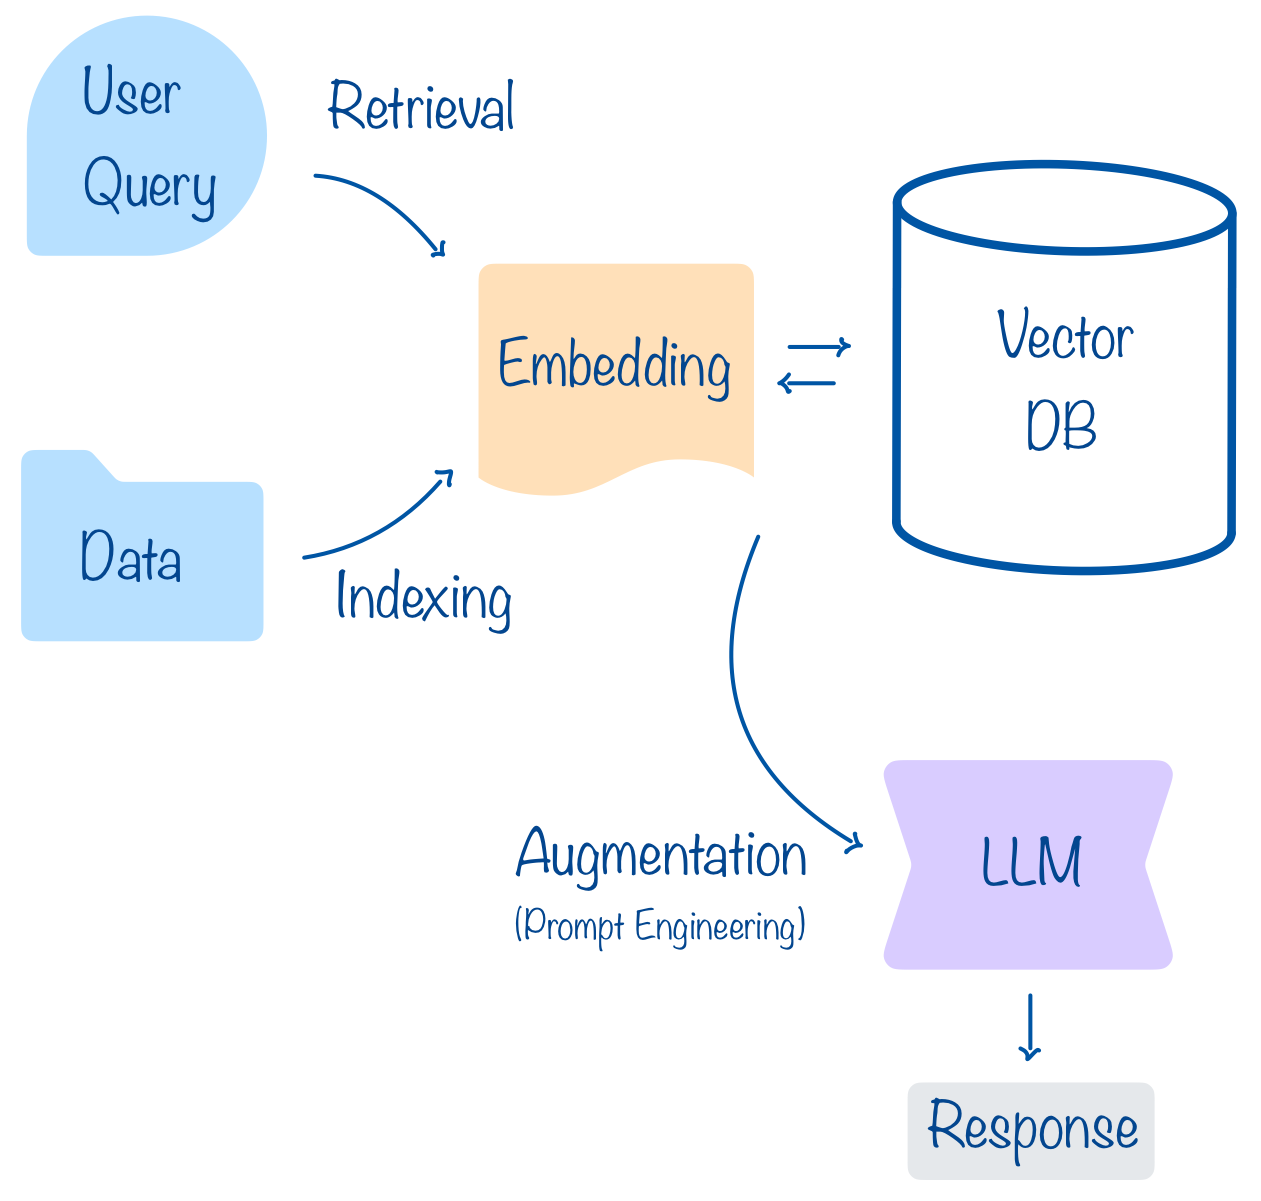
\includegraphics[width=0.7\textwidth]{resources/rag.png}
      \end{center}
  \end{columns}

  \vspace{8pt}
  {\footnotesize\color{NoteGray} Mechanistically, RAG is prompt engineering with retrieval --- dynamic ICL for knowledge grounding.}

  \vspace{6pt}
  {\footnotesize\color{AtlasCool} \textbf{Explore more:} \hyperlink{rag-variants}{RAG Variants} $\mid$ \hyperlink{vector-db}{Vector Databases \& Similarity Search}}

  \note{
    \footnotesize
    \textbf{Citation:} Lewis et al., ``Retrieval-Augmented Generation for Knowledge-Intensive NLP Tasks,'' NeurIPS 2020.\\[4pt]
    RAG combines parametric (model weights) and non-parametric (document index) memory. The key insight: knowledge can be updated without retraining by just updating the index.

    \textbf{The diagram:} Shows the full RAG pipeline. Data (documents) goes through indexing and embedding into a vector DB. When a user query arrives, it's also embedded, retrieval finds relevant chunks from the DB, those chunks get injected into the prompt (augmentation = prompt engineering), and the LLM generates a response grounded in the retrieved context.

    \textbf{Example (for delivery):} ``What were Anthropic's key findings in their interpretability paper?'' $\rightarrow$ embed query $\rightarrow$ retrieve top-K similar passages from paper DB $\rightarrow$ inject into context $\rightarrow$ answer grounded in retrieved text.

    \textbf{Relationship to ICL:} RAG uses the same context-window mechanism as ICL, but the injected content is retrieved documents (dynamic, query-dependent) rather than hand-written task examples (static). Think of it as ``dynamic ICL for knowledge grounding.''
  }
\end{frame}

% ---------------- Section 2 Summary: When to Use What ----------------
\begin{frame}{Summary: When to Use What}
  \small
  \begin{center}
  \footnotesize
  \begin{tabular}{p{2.8cm}ccc}
    \toprule
    \textbf{Criterion} & \textbf{Prompt Eng.} & \textbf{RAG} & \textbf{Domain SFT} \\
    \midrule
    Modifies weights? & No & No & \textbf{Yes} \\
    Upfront cost & None & Index build & \textbf{High (data + training)} \\
    Per-request cost & High (examples) & Medium (retrieval) & \textbf{Low (short prompts)} \\
    Update latency & Instant & Instant & Retrain \\
    Best for & Task steering & \textbf{Knowledge} & \textbf{Behavior} \\
    Reliability & Can drift & Depends on retrieval & \textbf{Durable (in weights)} \\
    \bottomrule
  \end{tabular}
  \end{center}

  \vspace{6pt}
  {\scriptsize\color{NoteGray} \textit{Prompt Engineering includes:} zero-shot instructions, few-shot ICL, chain-of-thought, role-playing, format specs, rules}

  \vspace{6pt}
  \begin{noteframe}
    \textbf{Rule of thumb:}
    \begin{itemize}[itemsep=2pt,topsep=2pt]
      \item \textbf{Quick iteration / low volume} $\rightarrow$ Prompt Engineering
      \item \textbf{Knowledge} (facts, documents that change) $\rightarrow$ RAG
      \item \textbf{Behavior} (format, style, reasoning) $\rightarrow$ SFT
      \item \textbf{Production} $\rightarrow$ SFT for behavior + RAG for knowledge
    \end{itemize}
  \end{noteframe}

  \note{
    \footnotesize
    This is the decision framework:

    \textbf{Prompt Engineering:} Use when iterating quickly, experimenting, or handling low-volume tasks. Zero upfront cost, instant changes, but you pay per request and behavior can be unreliable.

    \textbf{RAG:} Use when you need the model to \emph{know} different things (facts, documents). Knowledge lives in the index---swap documents and knowledge changes instantly without retraining. Best for evolving knowledge bases.

    \textbf{SFT:} Use when you need the model to \emph{act} differently (behavior, format, reasoning style). Bakes the change into weights---high upfront cost but durable and cheap per request.

    \textbf{Production systems:} Often combine SFT for behavior + RAG for dynamic knowledge. For example, SFT to teach the model your company's output format and reasoning style, RAG to ground answers in your current product docs.

    \textbf{Note on the table:} Prompt Engineering now encompasses all six techniques from the previous slide (zero-shot, ICL, CoT, role-playing, format specs, rules). ICL is no longer listed separately---it's one tool in the prompt engineering toolkit.
  }
\end{frame}

% ================================================================================
% SECTION 3: PEFT METHODS --- HOW TO DO DOMAIN SFT
% ================================================================================

% ---------------- Why Not Full Fine-Tuning? ----------------
\begin{frame}{Why Not Full Fine-Tuning?}
  \small
  \textbf{Full fine-tuning} = update every parameter in the model.

  \vspace{6pt}
  \textbf{Problems at scale:}
  \begin{itemize}
    \item \textbf{Memory:} GPT-3 175B needs $\sim$700GB VRAM just for gradients + optimizer states
    \item \textbf{Catastrophic forgetting:} model loses general capabilities when overtrained on narrow data
    \item \textbf{Storage:} need a separate 175B-parameter checkpoint per task/customer
    \item \textbf{Cost:} full training runs are expensive to repeat
  \end{itemize}

  \vspace{8pt}
  \begin{goodbox}
    \textbf{Solution: Parameter-Efficient Fine-Tuning (PEFT)}\\[3pt]
    Freeze most of the model; train only a small set of new or selected parameters.

    \vspace{3pt}
    {\footnotesize\color{NoteGray} PEFT is still SFT---same loss function, same training data. Only the \emph{scope} of what gets updated changes.}
  \end{goodbox}

  \note{
    \footnotesize
    The key insight: we don't need to update every parameter. Most of the model's knowledge is already useful; we just need to steer it slightly. PEFT methods exploit this by keeping the base model frozen and training a small ``adapter'' on top.
  }
\end{frame}

% ---------------- LoRA ----------------
\begin{frame}{LoRA: Low-Rank Adaptation}
  \small
  \textbf{Core idea} \textit{(Hu et al., 2021):} Weight updates are often low-rank---decompose $\Delta W$ into two small matrices.

  \vspace{4pt}
  \begin{center}
  \begin{tikzpicture}[font=\small]
    \node[draw, fill=gray!15, minimum width=2cm, minimum height=1.5cm, align=center] (W) {$W_0$\\(frozen)};
    \node[right=0.4cm of W] (plus) {\Large $+$};
    \node[draw, fill=AtlasCool!30, minimum width=0.6cm, minimum height=1.5cm, right=0.4cm of plus] (B) {$B$};
    \node[right=0.1cm of B] (times) {$\times$};
    \node[draw, fill=AtlasCool!30, minimum width=1.2cm, minimum height=0.5cm, right=0.1cm of times] (A) {$A$};
    \node[right=0.4cm of A] (eq) {$=$};
    \node[draw, fill=AtlasWarm!20, minimum width=2cm, minimum height=1.5cm, right=0.4cm of eq] (Wnew) {$W_{new}$};
  \end{tikzpicture}
  \end{center}

  \vspace{2pt}
  \begin{gather*}
    W_{new} = W_0 + \frac{\alpha}{r} B A, \quad A \in \mathbb{R}^{r \times d_{in}},\ B \in \mathbb{R}^{d_{out} \times r}
  \end{gather*}

  \only<1>{
  \vspace{2pt}
  \textbf{Key properties:}
  \begin{itemize}
    \item \textbf{Trainable params:} $\sim$0.01\% of full model (rank $r$ typically 4--64)
    \item \textbf{Memory:} 3$\times$ less GPU memory than full fine-tuning
    \item \textbf{Inference:} merge $BA$ into $W_0$ $\rightarrow$ \textbf{zero added latency}
    \item \textbf{Performance:} matches or exceeds full fine-tuning on many tasks
  \end{itemize}
}

\only<2->{
  \vspace{4pt}
  \begin{noteframe}
    \textbf{Which weights to adapt?}\\[2pt]
    {\footnotesize
    \textbf{Targeted:} LoRA applied per-weight-matrix, each gets its own $(A, B)$ pair\\
    \textbf{Attention first:} $W_q$, $W_k$, $W_v$, $W_o$ (standard targets)\\
    \textbf{MLP optional:} larger, holds world knowledge; costs more but helps when task needs new knowledge
    }
  \end{noteframe}
}
\end{frame}

\note{
    \footnotesize
    \textbf{Citation:} Hu et al., ``LoRA: Low-Rank Adaptation of Large Language Models,'' 2021.\\[4pt]
    The key insight: the weight \emph{change} $\Delta W$ during fine-tuning has low intrinsic rank. Instead of storing/training all of $\Delta W$, decompose it as $BA$ where $r \ll \min(d_{in}, d_{out})$. At inference, merge into $W_0$ so there's no runtime cost.

    \textbf{What is $\alpha$ and why normalize by $r$?}\\[3pt]
    $\alpha$ is a \textbf{scaling hyperparameter} that controls the magnitude of the LoRA update relative to the frozen weights $W_0$. The factor $\frac{\alpha}{r}$ in the formula $W_{new} = W_0 + \frac{\alpha}{r} BA$ serves two purposes:\\[3pt]
    (1) \textbf{Rank-independent scale}: Dividing by $r$ keeps the update magnitude roughly constant across different rank choices. Without this, doubling $r$ would double the update scale (since $BA$ has more capacity), making hyperparameter tuning unstable. With $\frac{\alpha}{r}$, you can change $r$ without re-tuning $\alpha$.\\[3pt]
    (2) \textbf{Initialization-agnostic learning rate}: $A$ is initialized with small random values, $B$ with zeros, so $BA$ starts near zero. The $\frac{\alpha}{r}$ scaling means you can set $\alpha$ (typically 8, 16, or 32) independently of the learning rate, and the effective contribution of LoRA grows predictably as training progresses.\\[3pt]
    In practice, $\alpha$ is often set equal to $r$ (so $\frac{\alpha}{r} = 1$) or kept fixed at a small multiple of $r$ (e.g., $\alpha = 2r$). This is a design choice to decouple the rank hyperparameter from the scale hyperparameter.
}

\note{
    \textbf{Which weight matrices to target.} In the transformer architecture, multi-head attention has four key weight matrices:
    \begin{itemize}[itemsep=1pt,topsep=2pt]
      \item $W_q$ (query projection) --- maps input to query vectors
      \item $W_k$ (key projection) --- maps input to key vectors
      \item $W_v$ (value projection) --- maps input to value vectors
      \item $W_o$ (output projection) --- combines the outputs from all attention heads back into the model's hidden dimension. After each attention head computes its own weighted sum of values, $W_o$ projects the concatenated head outputs back to the residual stream.
    \end{itemize}
    These four matrices determine \emph{what} the model attends to (queries and keys) and \emph{what information} it extracts (values and output combination). Adapting them steers attention patterns without retraining the entire model.
  }

  \note{
    \footnotesize
    \textbf{MLP adaptation.} The MLP layers (feed-forward networks) have their own weight matrices ($W_{up}$, $W_{down}$) that are larger and encode more factual knowledge. Adapting them costs more parameters but can be necessary when the task requires new knowledge pathways, not just attention steering.

    Standard practice: adapt attention matrices only (cheaper, often sufficient). Add MLP adaptation if the task needs new factual knowledge or reasoning patterns.
  }

% ---------------- PiSSA ----------------
\begin{frame}{LoRA Variants: PiSSA (SVD-Based Initialization)}
  \small
  \textbf{Problem with vanilla LoRA:} $A$ initialized with Gaussian noise, $B$ with zeros $\rightarrow$ slow convergence.

  \vspace{6pt}
  \textbf{PiSSA} \textit{(Meng et al., 2025):} Initialize adapters with the \textbf{principal singular components} of $W_0$ itself.

  \vspace{4pt}
  \begin{center}
  \footnotesize
  \begin{tikzpicture}[font=\scriptsize]
    \node[draw, minimum width=2cm, minimum height=1.2cm, align=center] (W) {$W_0$};
    \node[right=0.3cm of W] (svd) {SVD};
    \draw[-Stealth] (W) -- (svd);
    \node[draw, fill=AtlasCool!30, minimum width=0.5cm, minimum height=1.2cm, right=0.3cm of svd, align=center] (A) {$A$\\(top-$r$)};
    \node[right=0.1cm of A] (plus) {$+$};
    \node[draw, fill=gray!15, minimum width=1.5cm, minimum height=1.2cm, right=0.1cm of plus, align=center] (Wres) {$W^{res}$\\(frozen)};
  \end{tikzpicture}
  \end{center}

  \vspace{4pt}
  \textbf{Results:}
  \begin{itemize}
    \item Gemma-7B on GSM8K: PiSSA \textbf{77.7\%} vs.\ LoRA 74.5\% (+3.2\%)
    \item LLaMA-3-70B with 4-bit quant: QPiSSA \textbf{86.1\%} vs.\ QLoRA 81.7\% (+4.4\%)
    \item Initialization cost: seconds (fast SVD), negligible vs.\ training time
  \end{itemize}

  \vspace{4pt}
  {\footnotesize\color{NoteGray} Same architecture as LoRA---drop-in replacement. The only change is \emph{how} $A$ and $B$ are initialized.}

  \note{
    \footnotesize
    \textbf{Citation:} Meng et al., ``PiSSA: Principal Singular Values and Singular Vectors Adaptation of Large Language Models,'' 2025.\\[4pt]
    The intuition: LoRA trains the ``noise'' part; PiSSA trains the ``principal'' part. By initializing adapters with the top-$r$ singular components, PiSSA starts closer to the optimal solution and converges faster.

    \textbf{How SVD initialization works:}\\[3pt]
    (1) Compute SVD of the frozen weight matrix: $W_0 = U \Sigma V^T$\\[3pt]
    (2) Extract the \textbf{top-$r$ singular components}: $A_{init} = \Sigma_r V_r^T$ and $B_{init} = U_r$, where $\Sigma_r$ is the diagonal matrix of the $r$ largest singular values, and $U_r$, $V_r$ are the corresponding left/right singular vectors.\\[3pt]
    (3) The \textbf{trainable LoRA part} is initialized to $(B_{init}, A_{init})$ --- these $r$ components capture the most important directions of $W_0$ and will be updated during training.\\[3pt]
    (4) The \textbf{frozen residual} is $W^{res} = W_0 - B_{init} A_{init}$ --- this is the remainder after removing the top-$r$ components. $W^{res}$ stays frozen throughout training.\\[3pt]
    (5) During training: $W_{new} = W^{res} + BA$, where $(B, A)$ start from $(B_{init}, A_{init})$ and are updated by gradient descent.\\[3pt]
    
  }

\note{
    \footnotesize

  \textbf{Key insight:} By initializing the trainable part with the principal components (highest singular values = most variance), PiSSA starts training from a better initialization than random noise. The frozen residual holds the less-important directions that don't need adaptation.
}
\end{frame}

% ---------------- Other PEFT Families ----------------
\begin{frame}{Other PEFT Families}
  \small
  \begin{columns}[t]
    \column{0.32\textwidth}
    \textbf{\color{AtlasWarm}Adapters}\\
    \scriptsize\textit{(Houlsby et al., 2019)}\\[4pt]
    \footnotesize
    Insert small bottleneck layers \emph{inside} transformer blocks.

    \vspace{4pt}
    \begin{center}
    \begin{tikzpicture}[font=\tiny, node distance=0.15cm]
      \node[draw, minimum width=1cm, minimum height=0.4cm] (down) {Down};
      \node[draw, minimum width=1cm, minimum height=0.4cm, below=of down] (nl) {ReLU};
      \node[draw, minimum width=1cm, minimum height=0.4cm, below=of nl] (up) {Up};
      \draw[-Stealth] (down) -- (nl);
      \draw[-Stealth] (nl) -- (up);
    \end{tikzpicture}
    \end{center}

    \vspace{2pt}
    $\sim$3\% params per task.\\
    Adds inference latency.

    \column{0.32\textwidth}
    \textbf{\color{AtlasCool}Prefix-Tuning}\\
    \scriptsize\textit{(Li \& Liang, 2021)}\\[4pt]
    \footnotesize
    Prepend learnable ``virtual tokens'' to keys/values in every layer.

    \vspace{4pt}
    \begin{center}
    \begin{tikzpicture}[font=\tiny]
      \node[draw, fill=AtlasCool!20, minimum width=0.6cm, minimum height=0.4cm] (p1) {$p_1$};
      \node[draw, fill=AtlasCool!20, minimum width=0.6cm, minimum height=0.4cm, right=0.05cm of p1] (p2) {$p_2$};
      \node[draw, minimum width=0.6cm, minimum height=0.4cm, right=0.05cm of p2] (x1) {$x_1$};
      \node[draw, minimum width=0.6cm, minimum height=0.4cm, right=0.05cm of x1] (x2) {$x_2$};
    \end{tikzpicture}
    \end{center}

    \vspace{2pt}
    $\sim$0.1\% params.\\
    No architecture change.

    \column{0.32\textwidth}
    \textbf{\color{NoteGray}Prompt Tuning}\\
    \scriptsize\textit{(Lester et al., 2021)}\\[4pt]
    \footnotesize
    Learnable soft prompt at input layer only (not every layer).

    \vspace{4pt}
    Simpler than prefix-tuning.\\
    Scales with model size: ``closes the gap'' at 10B+ params.

    \vspace{4pt}
    $\sim$0.01\% params.\\
    Minimal overhead.
  \end{columns}

  \vspace{8pt}
  {\footnotesize\color{NoteGray} All methods freeze the base model and train only a small number of new parameters. Choice depends on your latency/memory constraints and how much expressiveness you need.}

  \end{frame}

  \note{
    \footnotesize
    \textbf{Adapters (Houlsby et al., ICML 2019):}\\[3pt]
    \textbf{What they are:} Small feedforward bottleneck modules inserted into each transformer layer, typically placed after the attention and MLP sublayers.\\[3pt]
    \textbf{Architecture:} Down-projection (e.g., $d \to d/8$), non-linearity (ReLU/GeLU), up-projection ($d/8 \to d$), with a residual connection around the adapter. Base model weights stay frozen; only adapter parameters are trained.\\[3pt]
    \textbf{What's trained:} The two projection matrices in each adapter module. Typically $\sim$3--4\% of total params (per task).\\[3pt]
    \textbf{Tradeoff:} Higher expressiveness than LoRA (dedicated network per layer), but adds inference latency since adapters are sequential modules in the forward pass. LoRA merges into weights at deploy time; adapters cannot.\\[3pt]
    \textbf{Results:} Within 0.4\% of full fine-tuning on GLUE benchmarks.
  }
    \note{
    \footnotesize

    \textbf{Prefix-Tuning (Li \& Liang, ACL 2021):}\\[3pt]
    \textbf{What it is:} Prepend learnable ``virtual token'' embeddings to the key and value projections in every transformer layer. These act like a soft prompt that conditions the entire model's behavior.\\[3pt]
    \textbf{How it works:} At each layer, instead of just attending to the real input tokens, the model also attends to a fixed-length sequence of learned prefix vectors. The prefixes are task-specific; base model is frozen.\\[3pt]
    \textbf{What's trained:} The prefix parameters (embeddings for the virtual tokens) at every layer. Typically $\sim$0.1\% of total params.\\[3pt]
    \textbf{Tradeoff:} Very parameter-efficient, no architecture change, but reduces effective context window (prefix tokens take up space). Works better in low-data regimes than full fine-tuning.\\[3pt]
    \textbf{Difference from Prompt Tuning:} Prefix-Tuning adds prefixes at \emph{every layer}; Prompt Tuning only at the input.
    }
    \note{
    \footnotesize
    \textbf{Prompt Tuning (Lester et al., EMNLP 2021):}\\[3pt]
    \textbf{What it is:} Learn a small set of continuous ``soft prompt'' embeddings that are prepended to the input sequence. Only the input layer is affected; no per-layer conditioning.\\[3pt]
    \textbf{How it works:} Instead of hand-writing discrete prompt text (``You are a helpful assistant\ldots''), learn K embedding vectors that get concatenated with the input token embeddings. The model processes them as if they were real tokens, but they're optimized by gradient descent, not discrete text.\\[3pt]
    \textbf{What's trained:} Just the soft prompt embeddings. Typically $\sim$0.01\% of total params ($\sim$20--100 tokens' worth).\\[3pt]
    \textbf{Key finding:} Performance gap vs. full fine-tuning shrinks dramatically as model size increases. At 10B+ parameters, prompt tuning matches full FT with 100$\times$ fewer trained params.\\[3pt]
    \textbf{Tradeoff:} Extremely cheap, but less expressive than adapters/LoRA. Best for very large models where capacity is abundant.
  }


% ---------------- Task Arithmetic ----------------
\begin{frame}{Task Arithmetic: Combining Adapters}
  \small
  \textbf{Core idea} \textit{(Ilharco et al., 2023):} A \textbf{task vector} = fine-tuned weights $-$ pretrained weights.

  \vspace{4pt}
  \begin{center}
  \begin{tikzpicture}[font=\small, node distance=0.3cm]
    \node[draw, minimum width=1.8cm, minimum height=0.8cm] (pre) {$\theta_{pre}$};
    \node[right=0.5cm of pre] (arrow) {fine-tune on task $A$};
    \node[draw, minimum width=1.8cm, minimum height=0.8cm, right=0.5cm of arrow] (ft) {$\theta_{ft}^A$};
    \draw[-Stealth] (pre) -- (arrow);
    \draw[-Stealth] (arrow) -- (ft);

    \node[below=0.6cm of arrow] (tau) {$\tau_A = \theta_{ft}^A - \theta_{pre}$};
  \end{tikzpicture}
  \end{center}

  \vspace{4pt}
  \textbf{Operations on task vectors:}
  \begin{itemize}
    \item \textbf{Negation:} $\theta_{pre} - \tau_A$ $\rightarrow$ \emph{reduces} performance on task $A$
    \item \textbf{Addition:} $\theta_{pre} + \tau_A + \tau_B$ $\rightarrow$ improves on \emph{both} $A$ and $B$
    \item \textbf{Analogy:} ``$A$ is to $B$ as $C$ is to $D$'' $\rightarrow$ combine $\tau_A$, $\tau_B$, $\tau_C$ to improve on $D$
  \end{itemize}

  \vspace{6pt}
  \textbf{No retraining needed}---just arithmetic on saved weight deltas.

  {\footnotesize\color{NoteGray} Works with LoRA too: each adapter is a task vector you can combine post-hoc.}

  \note{
    \footnotesize
    \textbf{Citation:} Ilharco et al., ``Editing Models with Task Arithmetic,'' ICLR 2023.

    The insight: fine-tuning creates a direction in weight space that encodes ``how to do this task.'' These directions can be added/subtracted like vectors. This enables multi-task models without multi-task training.

    \textbf{Analogy operation, precisely:} ``$A$ is to $B$ as $C$ is to $D$'' computes $\theta_{pre} + (\tau_B - \tau_A + \tau_C)$ to improve on task $D$. The transformation from $A$ to $B$ (captured by $\tau_B - \tau_A$) is applied to $C$ to predict $D$---same structure as word2vec's ``King - Man + Woman = Queen.''
  }


  \note{
    \footnotesize
    \textbf{Mathematical Intuition.}

    \textbf{Linear Mode Connectivity (LMC):} While neural network loss landscapes are highly non-convex, models initialized and fine-tuned from the exact same pre-trained checkpoint remain in the same wide, flat optimization basin.

    \textbf{Local Linearity:} Because the displacement during fine-tuning ($\tau$) is very small relative to the scale of the pre-trained weights ($\theta_{pre}$), the models remain in a locally linear region of the tangent space. Consequently, interpolating the weights linearly interpolates the function outputs.
  }
\end{frame}

% ---------------- Advanced Weight Merging Techniques ----------------
\begin{frame}{Advanced Weight Merging Techniques}
  \small
  \textbf{Problem:} Naive addition of task vectors causes interference---parameter conflicts between tasks.

  \vspace{6pt}
  \begin{center}
  \footnotesize
  \setlength{\tabcolsep}{5pt}
  \begin{tabular}{p{2.0cm}p{4.5cm}p{4.0cm}}
    \toprule
    \textbf{Method} & \textbf{How It Works} & \textbf{Key Benefit} \\
    \midrule
    \textbf{SLERP} & Spherical interpolation---preserves weight norm along a curved path & No magnitude squashing \\
    \textbf{TIES-Merging} & (1) Trim small deltas (2) Elect dominant sign (3) Merge agreeing params & Resolves sign conflicts \\
    \textbf{DARE} & Drop 90\% of deltas randomly, rescale survivors by $1/(1-p)$ & Extreme sparsity $\rightarrow$ less interference \\
    \bottomrule
  \end{tabular}
  \end{center}

  % \vspace{8pt}
  % \textbf{SLERP formula} (for $t \in [0,1]$ and angle $\Omega$ between $\theta_1$, $\theta_2$):
  % \begin{gather}
  % \theta_{merged} = \frac{\sin((1-t)\Omega)}{\sin(\Omega)}\theta_1 + \frac{\sin(t\Omega)}{\sin(\Omega)}\theta_2
  % \end{gather}

  % \vspace{4pt}
  % {\footnotesize\color{NoteGray} Linear interpolation: $\theta_{merged} = (1-t)\theta_1 + t\theta_2$ --- simple but squashes magnitude if vectors diverge.}
\end{frame}

\note{
  \footnotesize
  \textbf{Why these matter:} When combining multiple specialized models (e.g., a math expert + a code expert), their task vectors often point in conflicting directions for the same parameter. Naive addition averages them, which can degrade both capabilities.

  \textbf{SLERP:} Standard linear interpolation treats weight vectors as points in Euclidean space. If two vectors point in different directions, their average has smaller magnitude. SLERP interpolates along the surface of a hypersphere, keeping the norm constant throughout the path---like rotating from one vector to the other.

  \textbf{TIES-Merging:} Addresses three problems: (a) many small weight changes are noise, (b) tasks may push the same parameter in opposite directions (sign conflict), (c) averaging conflicting signs cancels them out. TIES trims noise, votes on the dominant direction per parameter, then merges only the changes that agree with the vote.

  \textbf{DARE:} Inspired by dropout and lottery tickets. Most fine-tuning deltas are redundant---only a sparse subset matters. By randomly dropping most deltas and rescaling survivors, you force the merge to rely on the strongest, most robust changes from each task, reducing interference.
}

% ---------------- Applications: Unlearning and Safety ----------------
\begin{frame}{Applications: Unlearning and Safety}
  \small
  Task vectors enable \textbf{editing models without retraining}.

  \vspace{8pt}
  \begin{columns}[t]
    \column{0.48\textwidth}
      \begin{tcolorbox}[colback=AtlasWarm!10, colframe=AtlasWarm, boxrule=0.5pt, arc=2pt, boxsep=3pt, left=3pt, right=3pt, top=3pt, bottom=3pt, title={\footnotesize\textbf{Targeted Forgetting}}]
        \footnotesize
        \textbf{Goal:} Remove toxic, copyrighted, or private data from a trained model.

        \vspace{4pt}
        \textbf{Method:}
        \begin{itemize}[itemsep=1pt,topsep=2pt,label=$\triangleright$]
          \item Fine-tune model on unwanted data $\rightarrow$ $\theta_{bad}$
          \item Compute $\tau_{bad} = \theta_{bad} - \theta_{base}$
          \item Apply: $\theta_{new} = \theta_{base} - \lambda \tau_{bad}$
        \end{itemize}

        \vspace{4pt}
        Pushes weights \emph{away} from the learned representations.
      \end{tcolorbox}

    \column{0.48\textwidth}
      \begin{tcolorbox}[colback=AtlasCool!10, colframe=AtlasCool, boxrule=0.5pt, arc=2pt, boxsep=3pt, left=3pt, right=3pt, top=3pt, bottom=3pt, title={\footnotesize\textbf{Alignment without RLHF}}]
        \footnotesize
        \textbf{Goal:} Add safety guardrails to an unaligned model without access to RLHF data.

        \vspace{4pt}
        \textbf{Method:}
        \begin{itemize}[itemsep=1pt,topsep=2pt,label=$\triangleright$]
          \item Isolate ``alignment'' task vector $\tau_{safe}$ from safe model
          \item Scale into unaligned base: $\theta_{new} = \theta_{base} + \lambda \tau_{safe}$
        \end{itemize}

        \vspace{4pt}
        Transfers safety properties across models.
      \end{tcolorbox}
  \end{columns}

  \vspace{8pt}
  {\footnotesize\color{NoteGray} Both leverage the linear structure of task vectors---behavior encoded as directions in weight space can be added, subtracted, or scaled.}
\end{frame}

\note{
  \footnotesize
  \textbf{Targeted Forgetting:} Traditional unlearning requires retraining from scratch on a filtered dataset (expensive, sometimes impossible if you've lost the original training data). Task arithmetic offers a computational shortcut: fit the unwanted data to measure its direction in weight space, then push away from that direction. Not perfect---the model might still retain indirect associations---but far cheaper than retraining.

  \textbf{Alignment without RLHF:} RLHF is expensive (human feedback, reward modeling, RL training). If you have one aligned model and one unaligned model (both from the same base), you can extract the ``alignment vector'' as $\tau_{safe} = \theta_{aligned} - \theta_{base}$, then inject it into a different unaligned checkpoint. This transfers safety behavior compositionally, without re-running RLHF. Particularly useful for quickly prototyping safe versions of new model variants.

  \textbf{Broader implications:} Task arithmetic treats model editing as a linear algebra problem. This opens up possibilities for fine-grained control (e.g., ``reduce toxicity by 50\% but keep sarcasm,'' ``add coding ability without losing creative writing'') that would be hard to achieve via traditional training objectives.
}

% ---------------- Section 3 Summary: PEFT Comparison ----------------
\begin{frame}{Summary: PEFT Method Comparison}
  \small
  \begin{center}
  \footnotesize
  \setlength{\tabcolsep}{4pt}
  \begin{tabular}{p{2.0cm}ccccc}
    \toprule
    \textbf{Method} & \textbf{Params} & \textbf{Memory} & \textbf{Inference} & \textbf{Where} & \textbf{Composable?} \\
    \midrule
    Full FT & 100\% & Very high & None & All & No \\
    \textbf{LoRA} & 0.01--0.1\% & 3$\times$ lower & \textbf{None} (merge) & Attention & \textbf{Yes} \\
    PiSSA & 0.01--0.1\% & 3$\times$ lower & \textbf{None} & Attention & Yes \\
    Adapters & 1--5\% & Medium & Added & Each layer & Yes \\
    Prefix-Tuning & 0.1\% & Low & Minimal & K/V cache & Yes \\
    Prompt Tuning & 0.01\% & Very low & None & Input only & Yes \\
    \bottomrule
  \end{tabular}
  \end{center}

  \vspace{8pt}
  \textbf{Practical defaults:}
  \begin{itemize}
    \item \textbf{Start with LoRA} ($r$=8--32): best balance of efficiency and performance
    \item \textbf{Try PiSSA} if LoRA converges slowly: same cost, faster training
    \item \textbf{Use Adapters} if you need maximum expressiveness and can tolerate latency
    \item \textbf{Task Arithmetic} to combine multiple LoRA/adapters without retraining
  \end{itemize}

  \note{
    \footnotesize
    LoRA is the current default in industry due to zero inference overhead (weights can be merged). Adapters were the original PEFT method but add latency. Prefix/Prompt tuning are elegant but less flexible. The ecosystem (Hugging Face PEFT library, etc.) has converged on LoRA as the standard.
  }
\end{frame}

% ---------------- Conclusion ----------------
\begin{frame}{}
  % \begin{columns}[T]
  %   \begin{column}{0.48\textwidth}
  %     \footnotesize
  %     \textbf{SFT bridges} raw completion to instruction-following.

  %     \vspace{3pt}
  %     \begin{itemize}[itemsep=1pt,topsep=1pt]
  %       \item \textbf{Two purposes:} Alignment \& Domain
  %       \item \textbf{Quality $>$ quantity:} LIMA 1K beats 52K
  %       \item \textbf{Same loss, curated data:} masked CE
  %       \item \textbf{Alternatives:} prompting, RAG, PEFT
  %       \item \textbf{Not the end:} RLHF/DPO after
  %     \end{itemize}

  %     \vspace{5pt}
  %     {\scriptsize\color{NoteGray} \textbf{Rule of thumb:}\\RAG for knowledge, SFT for behavior,\\RL for preferences}
  %   \end{column}

    % \begin{column}{0.48\textwidth}
    %   \vspace{-8pt}
      \centering
      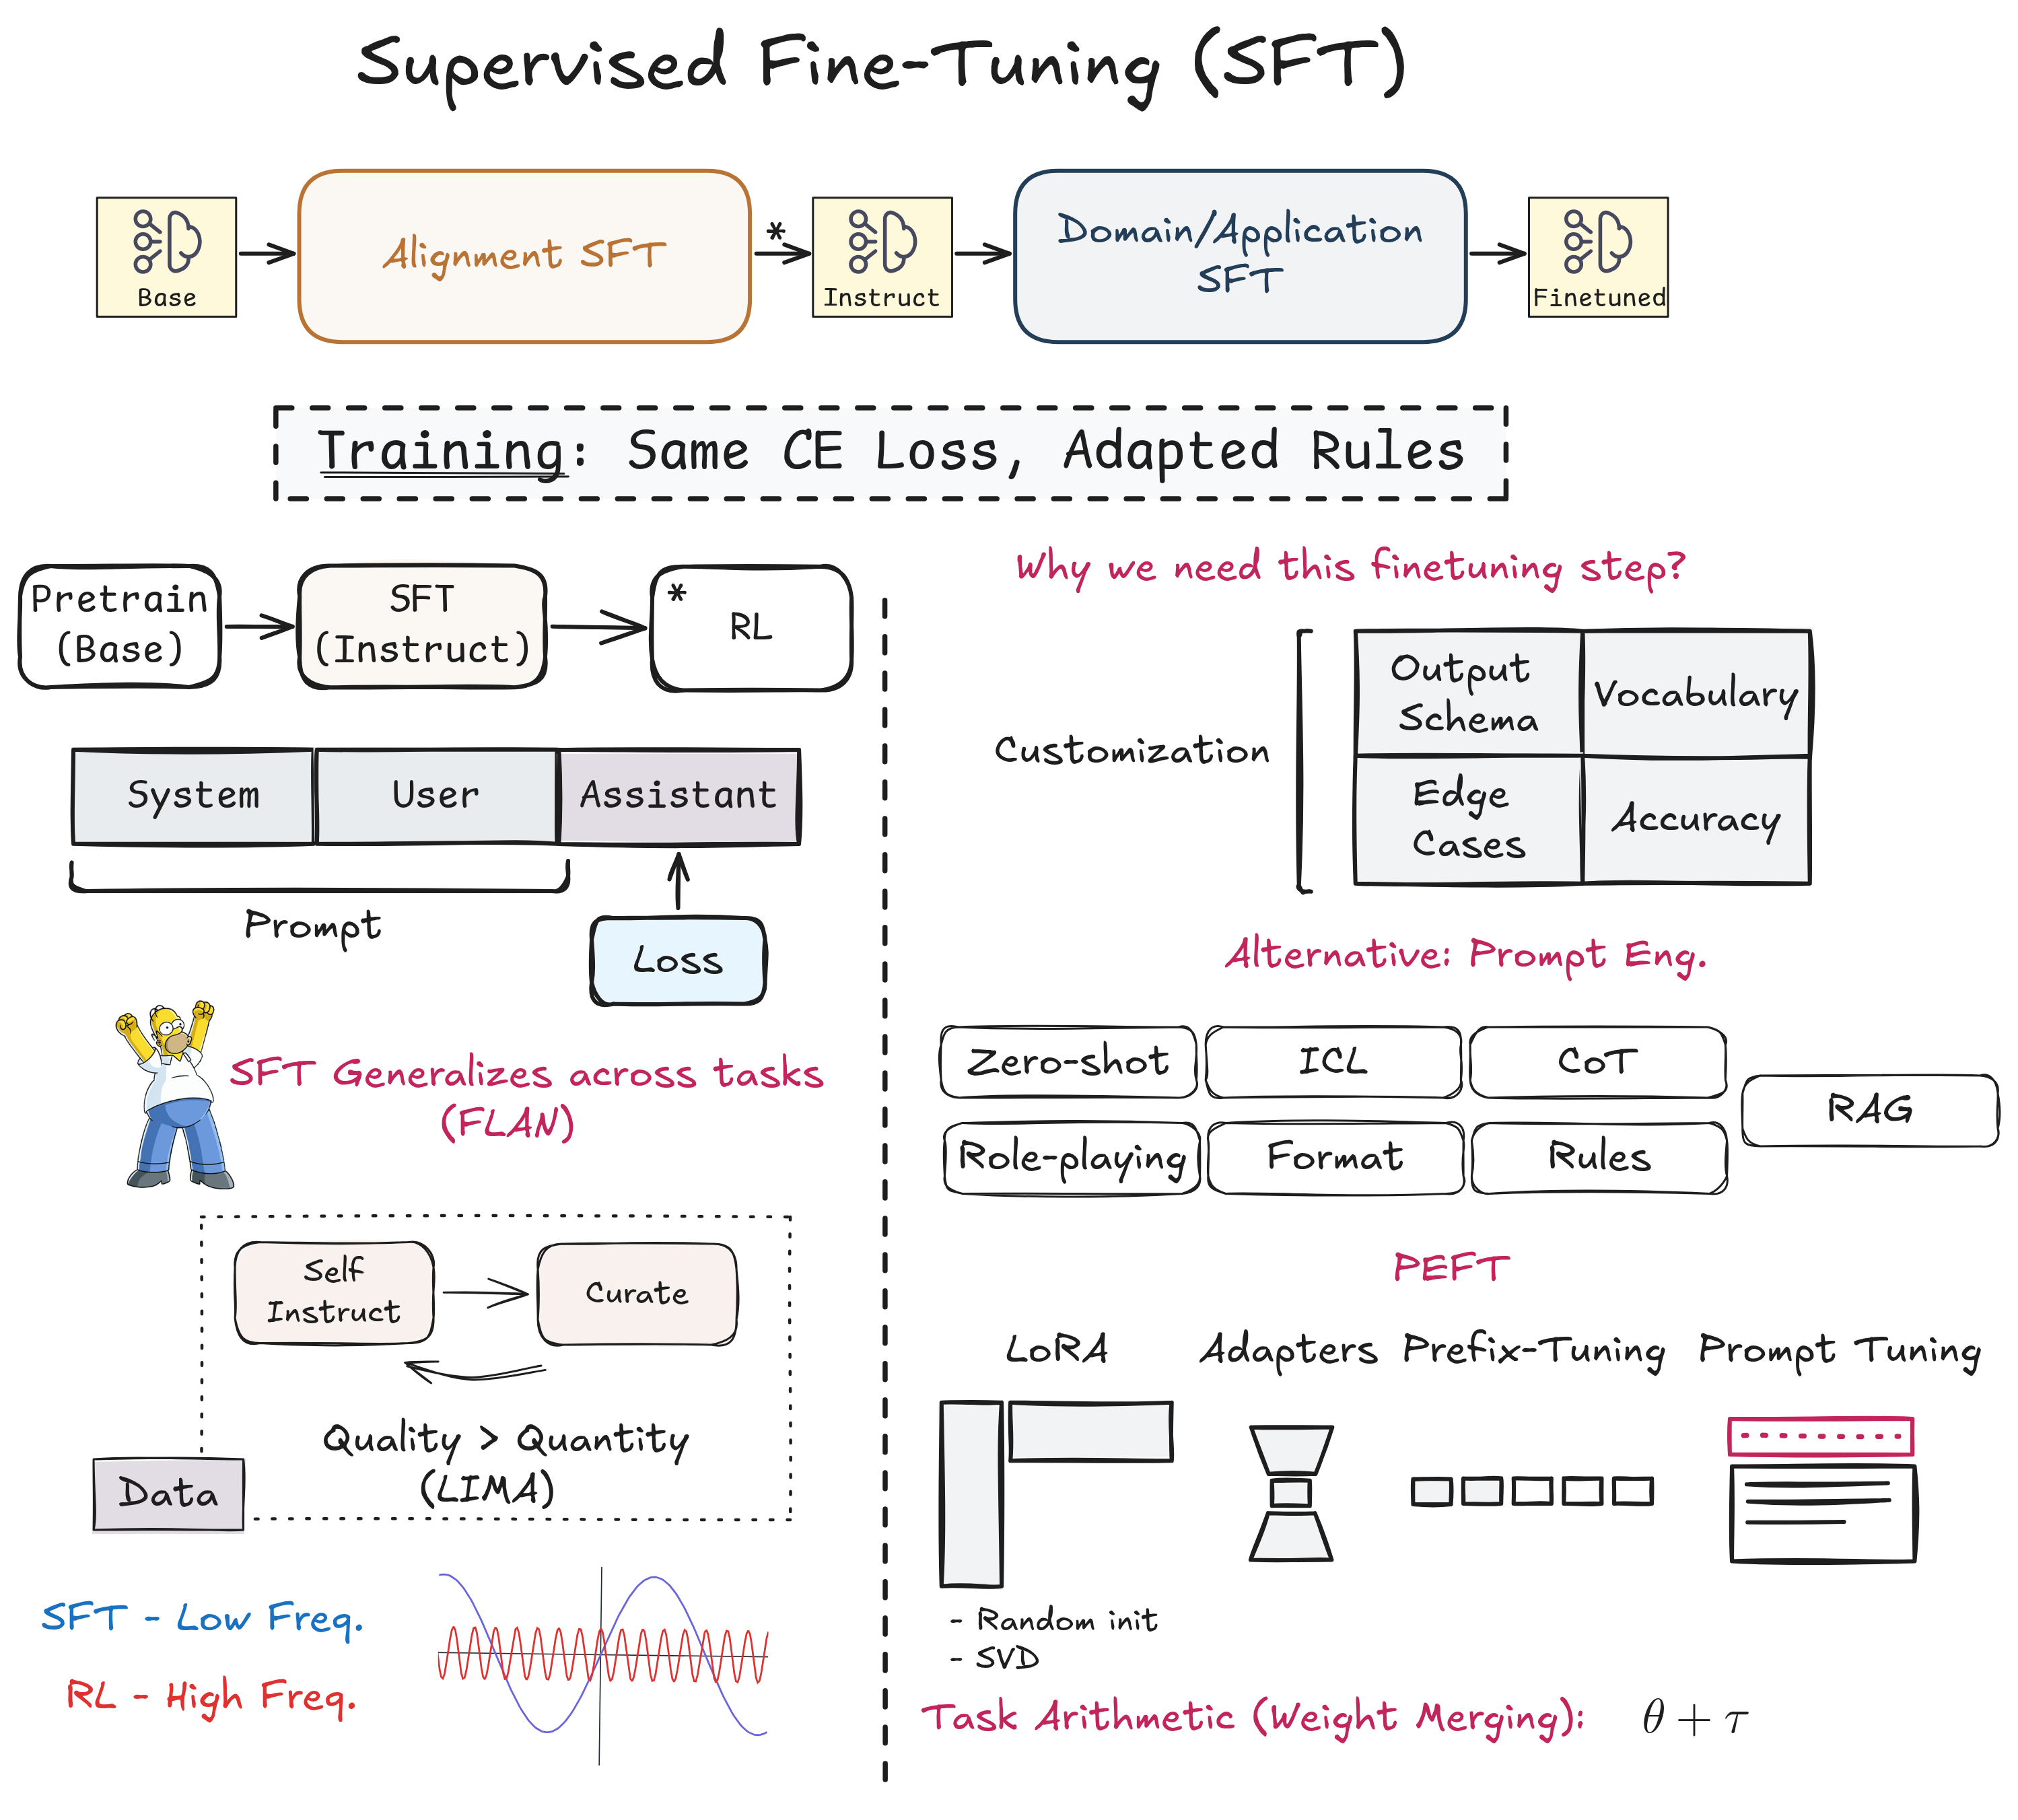
\includegraphics[width=0.7\textwidth]{map}
    % \end{column}
  % \end{columns}

  \note{
    \footnotesize
    \textbf{Delivery:} Tie it all together. SFT is one stage in a pipeline---it's not magic, just supervised learning on the right data. The real insight is understanding when to use it (behavior, format) vs. when alternatives (RAG for facts, prompt engineering for quick iteration) are better.

    The deck covered both purposes (alignment and domain), the mechanics (masked CE loss, chat templates), the quality-over-quantity insight (LIMA, Llama 3's curation), and the alternatives/variants (prompt engineering, RAG, PEFT). Now the audience should understand not just \emph{how} SFT works, but \emph{when} and \emph{why} to use it.

    \textbf{The map (right column):} Shows the full landscape we covered---the entire pipeline from pre-training through SFT to RL, the alternatives (prompt engineering, RAG), and the variants (PEFT/LoRA). Visual summary of all the decision points and tradeoffs discussed in the talk.
  }
\end{frame}

% ---------------- RAG Variants ----------------
\begin{frame}{RAG Variants: Active, Hierarchical, Graph-Based}
  \hypertarget{rag-variants}{}
  \small
  The basic RAG pattern has many extensions:

  \vspace{6pt}
  \begin{center}
  \footnotesize
  \begin{tabular}{p{2.2cm}p{4.0cm}p{4.0cm}}
    \toprule
    \textbf{Variant} & \textbf{Key Idea} & \textbf{Best For} \\
    \midrule
    \textbf{Self-RAG} \newline\scriptsize(Asai et al., 2023) & Model decides \emph{when} to retrieve; critiques own outputs & Reducing unnecessary retrieval \\
    \textbf{FLARE} \newline\scriptsize(Jiang et al., 2023) & Retrieves \emph{during} generation when confidence drops & Long-form generation \\
    \textbf{RAPTOR} \newline\scriptsize(Sarthi et al., 2024) & Hierarchical tree of summaries, not flat chunks & Multi-hop reasoning \\
    \textbf{Graph RAG} \newline\scriptsize(Edge et al., 2025) & Entity graph + community summaries & Complex entity relationships \\
    \bottomrule
  \end{tabular}
  \end{center}

  \vspace{6pt}
  {\footnotesize\color{NoteGray} All variants share the core idea: inject external knowledge at inference time rather than baking it into weights. Choice depends on your retrieval patterns and reasoning complexity.}

  \vspace{6pt}
  {\footnotesize\color{AtlasCool} \hyperlink{rag-main}{$\leftarrow$ Back to RAG}}
\end{frame}

\note{
  \footnotesize
  These variants address different limitations of basic RAG:

  \textbf{Self-RAG (Asai et al., 2023):} The model learns to decide \emph{when} to retrieve, not just blindly retrieving for every query. It also learns to critique its own outputs using special reflection tokens. Problem it solves: basic RAG retrieves on every query even when the model already knows the answer or when retrieval would add noise. Self-RAG adds a lightweight retrieval-gating mechanism trained into the model itself (via supervised fine-tuning on examples labeled with ``retrieve'' or ``don't retrieve'' decisions). It also generates critique tokens (``[IsRel]'', ``[IsSup]'', ``[IsUse]'') to self-assess whether retrieved docs are relevant, whether they support the generation, and whether the answer is useful.

  \textbf{FLARE (Jiang et al., 2023):} Forward-Looking Active REtrieval. Retrieves \emph{during} generation, not just once at the start. Problem it solves: in long-form generation (e.g., multi-paragraph answers), the initial query might not anticipate what knowledge will be needed later in the generation. FLARE monitors the model's confidence token-by-token (via probability thresholds) and triggers retrieval mid-stream when confidence drops. The retrieved content is injected into the context, and generation continues. Especially useful for open-ended tasks like writing reports or essays where the needed knowledge emerges as the generation unfolds.
}

\note{
  \footnotesize
  \textbf{RAPTOR (Sarthi et al., 2024):} Recursive Abstractive Processing for Tree-Organized Retrieval. Builds a hierarchical tree of document summaries instead of flat chunks. Problem it solves: flat-chunk retrieval (the basic RAG approach) struggles with multi-hop reasoning or questions that require synthesizing information scattered across many chunks. RAPTOR clusters similar chunks, generates summaries of each cluster, then recursively clusters and summarizes again, building a tree. At retrieval time, it can pull from both leaf chunks (fine-grained) and internal summaries (coarse-grained), giving the model access to both details and high-level overviews.

  \textbf{Graph RAG (Edge et al., 2025):} Builds an entity knowledge graph from the corpus (entities as nodes, relationships as edges) and uses community detection to generate summaries. Problem it solves: entity-heavy queries (``What are all the connections between X and Y?'') are hard for flat-chunk or even hierarchical RAG because the relationships are implicit across chunks. Graph RAG explicitly extracts entities and relationships, organizes them into a graph, detects communities (clusters of related entities), and retrieves both relevant subgraphs and community summaries. Best for knowledge bases with dense entity relationships (e.g., scientific papers, legal documents, social networks).
}

% % ================================================================================
% % ARCHIVE MARKER
% % ================================================================================

% \begin{frame}
%   \begin{center}
%     \vspace{2cm}
%     {\Huge\color{NoteGray} Archived From Here Down}

%     \vspace{1cm}
%     {\large The following slides are reference material from earlier drafts.}

%     \vspace{0.5cm}
%     {\footnotesize Not part of the main presentation.}
%   \end{center}
% \end{frame}

% % ================================================================================
% % ARCHIVED SLIDES (original Domain SFT content, kept for reference)
% % ================================================================================

% % ---------------- Prompt Engineering vs Domain SFT ----------------
% \begin{frame}{Prompt Engineering vs. Domain SFT}
%   \begin{center}
%   \small
%   \begin{tabular}{p{2.6cm}p{4.4cm}p{4.4cm}}
%     \toprule
%     \textbf{Metric} & \textbf{Prompt Engineering (Few-Shot)} & \textbf{Supervised Fine-Tuning (SFT)} \\
%     \midrule
%     Upfront Cost & \$0 --- immediate setup via API & High --- data collection + GPU rent \\
%     Cost Per Request & High --- paying for examples every time & Minimal --- short, clean prompts \\
%     Format Reliability & Weak --- model can drift or forget rules & Hardcoded --- baked into model weights \\
%     \bottomrule
%   \end{tabular}
%   \end{center}
%   \vspace{2pt}
%   {\footnotesize\color{NoteGray} Mostly a choice against \emph{domain} SFT specifically (recall slide 3) --- an already instruction-following model can often be steered by examples instead of retrained. Prompt engineering can also approximate alignment itself, but you pay for it on every request, and it's fragile; SFT bakes the behavior into the weights once.}
% \end{frame}

% % ---------------- A Third Axis: ICL & RAG ----------------
% \begin{frame}{A Third Axis: In-Context Learning \& RAG}
%   \small
%   \begin{center}
%   \begin{tikzpicture}[node distance=0.5cm, every node/.style={font=\scriptsize}]
%     \node[draw, rounded corners, minimum width=1.8cm, minimum height=1cm, align=center] (q) {Query};
%     \node[draw, rounded corners, fill=AtlasWarm!20, draw=AtlasWarm, minimum width=2.6cm, minimum height=1cm, align=center, right=of q] (r) {Retrieve\\relevant docs / examples};
%     \node[draw, rounded corners, minimum width=2.2cm, minimum height=1cm, align=center, right=of r] (i) {Inject into\\Context};
%     \node[draw, rounded corners, minimum width=2.6cm, minimum height=1cm, align=center, right=of i] (a) {Model Answers\\no weight update};
%     \draw[-Stealth] (q) -- (r);
%     \draw[-Stealth] (r) -- (i);
%     \draw[-Stealth] (i) -- (a);
%   \end{tikzpicture}
%   \end{center}
%   \vspace{6pt}
%   \begin{itemize}
%     \item \textbf{In-context learning:} few-shot examples or instructions placed directly in the prompt --- no training, forgotten the moment the request ends.
%     \item \textbf{RAG (Retrieval-Augmented Generation):} automates \emph{what} goes into that context, pulling relevant passages from a knowledge base instead of hand-picking examples.
%   \end{itemize}

%   RAG is a technique that allows LLMs to retrieve relevant information from a knowledge base.

%   \vspace{-2pt}
%   {\footnotesize\color{NoteGray} SFT bakes behavior into the weights --- durable, cheap per request, but paid for upfront. RAG/ICL instead change what's in the context --- cheap to update, but paid on every request. Rule of thumb: RAG for \emph{knowledge}, SFT for \emph{behavior}.}

%   \note{\color{red} For the RAG I can search for the slides I did for the RAG paper and take stuff from there. Convert the relevant diagrams to excalidraw instead of using the goodnotes versions.}

% \end{frame}

% % ---------------- Full FT vs PEFT (LoRA) ----------------
% \begin{frame}{Full Fine-Tuning vs. PEFT (LoRA)}
%   \begin{columns}[t]
%     \column{0.5\textwidth}
%       \textbf{\color{AtlasWarm}Full Fine-Tuning (FT)}\\[4pt]
%       \begin{center}
%       \begin{tikzpicture}
%         \foreach \x in {0,...,3} {
%           \foreach \y in {0,...,2} {
%             \node[draw, minimum size=0.7cm, fill=AtlasWarm!15] at (\x*0.75,-\y*0.75) {\scriptsize $\Delta\theta$};
%           }
%         }
%       \end{tikzpicture}
%       \end{center}
%       {\small Every parameter updates. High risk of catastrophic forgetting; massive VRAM for gradients + optimizer states.}
%     \column{0.5\textwidth}
%       \textbf{\color{AtlasCool}PEFT --- Variant, Not Alternative}\\[4pt]
%       \begin{center}
%       \begin{tikzpicture}[font=\small]
%         \node[draw, fill=gray!15, minimum width=1.6cm, minimum height=1.2cm] (frozen) {Frozen};
%         \node[right=0.3cm of frozen] (plus) {$+$};
%         \node[draw, fill=AtlasCool!20, minimum width=0.7cm, minimum height=1.2cm, right=0.3cm of plus] (A) {A};
%         \node[draw, fill=AtlasCool!35, minimum width=0.7cm, minimum height=0.5cm, right=0.3cm of A] (B) {B};
%       \end{tikzpicture}
%       \end{center}
%       {\small Still SFT --- same masked CE loss, same data. Only a tiny fraction of parameters (the LoRA matrices) actually train; the base model stays frozen.}
%   \end{columns}

%   \note{\color{red} I can say  that the LoRA is less expressive mapping but then is it a good or bad thing? less expressive is a form of regularization. Should check it before and check also if this is the most important point to mention here or are there other more/similarly important points.}
% \end{frame}

% % ---------------- LoRA Inside the Transformer ----------------
% \begin{frame}{LoRA Inside the Transformer}
  
%   \footnotesize
%   \begin{center}
%   \begin{tikzpicture}[node distance=0.25cm, font=\scriptsize]
%     \node[draw, rounded corners, minimum width=8.5cm, align=center, inner sep=3pt] (attn) {Multi-Head Self-Attention\\[2pt]
%       \tikz{
%         \node[draw, fill=AtlasWarm!25, draw=AtlasWarm, minimum width=0.8cm, minimum height=0.5cm] (wq) {$W_q$};
%         \node[draw, fill=AtlasWarm!25, draw=AtlasWarm, minimum width=0.8cm, minimum height=0.5cm, right=0.15cm of wq] (wk) {$W_k$};
%         \node[draw, fill=AtlasWarm!25, draw=AtlasWarm, minimum width=0.8cm, minimum height=0.5cm, right=0.15cm of wk] (wv) {$W_v$};
%         \node[draw, fill=AtlasWarm!25, draw=AtlasWarm, minimum width=0.8cm, minimum height=0.5cm, right=0.15cm of wv] (wo) {$W_o$};
%       }
%     };
%     \node[draw, rounded corners, minimum width=8.5cm, align=center, inner sep=3pt, below=0.2cm of attn] (mlp) {Feed-Forward (MLP)\\[2pt]
%       \tikz{
%         \node[draw, minimum width=1.1cm, minimum height=0.5cm] (wup) {$W_{up}$};
%         \node[draw, minimum width=1.1cm, minimum height=0.5cm, right=0.2cm of wup] (wdown) {$W_{down}$};
%       }
%     };
%   \end{tikzpicture}
%   \end{center}
%   \vspace{-10pt}
%   \begin{gather}
%     W_{\mathrm{new}} = W_0 + \frac{\alpha}{r}(B \times A), \quad A \in \mathbb{R}^{r \times d},\ B \in \mathbb{R}^{d \times r}
%   \end{gather}
%   \vspace{-14pt}
%   \begin{itemize}
%     \item \textbf{Targeted, not global:} each adapted matrix gets its own low-rank pair (A, B) --- LoRA is applied per-weight-matrix, not once to the whole model.
%     \item \textbf{Attention first:} $W_q$/$W_k$/$W_v$/$W_o$ are the standard targets --- they control \emph{what the model attends to}.
%     \item \textbf{MLP is optional:} larger, and holds more world knowledge --- costs more to adapt but helps when the task needs new knowledge pathways.
%   \end{itemize}

%   \note{\color{red} Not only Lora, also the SVD based, and perhaps other methods. I should see if I can find good survey or comparison or more relevant tools.\\
%   Don't forget to check in the end Dima's presentation and see if there are other points that I should include here.\\

%   Make sure you show how much parameters we use with lora compared to non lora and some measure on performance. 
%   }

% \end{frame}

% % ---------------- Retrieval-Augmented Generation (RAG) ----------------
% \begin{frame}{Retrieval-Augmented Generation (RAG)}
%   \small
%   RAG (Lewis et al., 2020) shifts the focus entirely away from parameter adaptation. Rather than
%   embedding domain knowledge into the model's internal weights via gradient updates, RAG
%   dynamically fetches relevant text chunks from an external vector database at inference time and
%   injects them directly into the prompt context.
%   \vspace{6pt}

%   \begin{center}
%   \footnotesize
%   \def\arraystretch{1.3}
%   \begin{tabular}{>{\raggedright\arraybackslash}p{1.9cm}>{\raggedright\arraybackslash}p{4.3cm}>{\raggedright\arraybackslash}p{4.3cm}}
%     \toprule
%     \textbf{Feature} & \textbf{\color{AtlasWarm}PEFT} & \textbf{\color{AtlasCool}RAG} \\
%     \midrule
%     Core Mechanism & Modifies internal neural weights. & Modifies the input prompt context. \\
%     Primary Strength & Teaching new formats, tone, syntax, or distinct reasoning patterns. & Injecting massive datasets of factual, proprietary, or highly dynamic knowledge. \\
%     Updating Knowledge & Requires re-running the optimization and training process. & Instantaneous database updates without touching the model. \\
%     Hallucination Risk & High; the model relies on parametric memory and may confidently invent facts. & Low; the model is explicitly grounded by the retrieved external context. \\
%     \bottomrule
%   \end{tabular}
%   \end{center}

%   \note{
%     \footnotesize
%     \textbf{Source.} Lewis et al., \emph{Retrieval-Augmented Generation for Knowledge-Intensive NLP
%     Tasks} (2020) --- combines a parametric generator with a non-parametric (retrieved) memory.

%     \color{red} Placeholder slide, pasted in as-is --- still needs to be reworked into the deck's
%     own visual style (currently a plain table, not TikZ/warmbox like the rest of the deck), checked
%     against the actual paper for accuracy, and positioned relative to the earlier ``A Third Axis:
%     ICL \& RAG'' slide (this may be redundant with it, or should replace/merge with it).
%   }

% \end{frame}

% ---------------- Vector Databases & Similarity Search ----------------
\begin{frame}{Vector Databases \& Similarity Search}
  \hypertarget{vector-db}{}
  \footnotesize
  \textbf{Approximate Nearest Neighbor (ANN) search} enables efficient retrieval at scale.

  \vspace{6pt}
  \textbf{Common similarity measures:}
  \begin{itemize}[itemsep=1pt,topsep=2pt]
    \footnotesize
    \item \textbf{Euclidean Distance} --- geometric distance in vector space
    \item \textbf{Cosine Similarity} --- angle between vectors (ignores magnitude)
    \item \textbf{Dot Product} --- combines magnitude and direction
  \end{itemize}

  \vspace{8pt}
  \textbf{Indexing methods} (sacrifice perfect accuracy for speed):

  \vspace{4pt}
  \begin{center}
  \scriptsize
  \setlength{\tabcolsep}{4pt}
  \begin{tabular}{p{1.2cm}p{1.5cm}p{4.0cm}p{5.0cm}}
    \toprule
    \textbf{Method} & \textbf{Core Idea} & \textbf{How it Works} & \textbf{Best For} \\
    \midrule
    HNSW & Graph & Navigates multi-layered graph to find neighbors & Performance \& accuracy-critical (common default) \\
    IVF & Clustering & Searches only within relevant vector clusters & Very large datasets, memory-constrained \\
    LSH & Hashing & Hashes similar vectors into same bucket & Massive scale, speed over perfect accuracy \\
    \bottomrule
  \end{tabular}
  \end{center}

  \vspace{4pt}
  {\footnotesize\color{NoteGray} Trade-off: exact search is $O(n)$; ANN methods achieve sub-linear query time with controllable accuracy loss.}

  \vspace{6pt}
  {\footnotesize\color{AtlasCool} \hyperlink{rag-main}{$\leftarrow$ Back to RAG}}
\end{frame}

\end{document}
